% Copyright (c) 2015 Daniele Masini - d.masini.it@gmail.com

\chapter{Trasformazioni geometriche piane}\label{chap:trasformazioni}

% \includegraphics[width=0.95\textwidth]{\folder img/danza_degli_storni.jpg}
%   \begin{center}
%     {\large ``La danza degli storni''}\par
%     Foto di \_Peck\_\par
%     \url{http://www.flickr.com/photos/_pek_/4113244536/}\par
%     Licenza: Creative Commons Attribution 2.0\par
%   \end{center}
% \newpage


\section{Generalità sulle trasformazioni geometriche piane}
\label{sect:generalita_trasformazioni}

\subsection{Introduzione e definizioni}

\begin{quote}
<<C'è una cosa straordinaria da vedere a Roma in questa fine 
d'autunno ed è il cielo gremito d'uccelli. Il terrazzo del signor 
Palomar è un buon punto d'osservazione [\ldots{}] Nell'aria viola del 
tramonto egli guarda affiorare da una parte del cielo un pulviscolo 
minutissimo, una nuvola d'ali che volano [\ldots{}] Quando si pensa 
agli uccelli migratori ci si immagina di solito una formazione di volo 
molto ordinata e compatta [\ldots{}] Quest'immagine non vale per gli 
storni, o almeno per questi storni autunnali nel cielo di Roma 
[\ldots{}]>>

\hfill{}Da \emph{Palomar} di Italo Calvino
\end{quote}

Il volo degli storni disegna nel cielo figure in continua 
trasformazione, come si può vedere dalle foto riportate nelle 
figure~\ref{fig:storni1} e~\ref{fig:storni2}.

\begin{figure*}[!htb]
\begin{center}
  \noindent\begin{minipage}{0.485\textwidth}
    \centering
    \includegraphics[width=\textwidth]{\folder img/danza_degli_storni.jpg}
    \caption{\emph{La danza degli storni}
      \protect\footnotemark}\label{fig:storni1}
  \end{minipage}
  \hspace{2mm}  
  \noindent\begin{minipage}{0.47\textwidth}
    \centering
    
\includegraphics[width=\textwidth]{\folder img/Auklet_flock_Shumagins_1986.jpg}
    \caption{\emph{Auklet flock, Shumagins 1986}\protect\footnotemark
            }\label{fig:storni2}
  \end{minipage}
\end{center}
\end{figure*}

\footnotetext[1]{foto di \_Peck\_, 
\url{http://www.flickr.com/photos/_pek_/4113244536/}.}
\footnotetext[2]{foto di D. Dibenski, 
\url{
http://commons.wikimedia.org/wiki/File:Auklet_flock_Shumagins_1986.jpg
}.}

%
% \begin{inaccessibleblock}[Figura: TODO]
%  \begin{figure}[!htb]
%  \begin{minipage}{0.4\textwidth}
%    \centering
%    
% \includegraphics[width=0.4\textwidth]{danza_degli_storni.jpg}
%    \caption{\emph{La danza degli storni}, foto di 
% \_Peck\_\\\url{http://www.flickr.com/photos/_pek_/4113244536/}}\label{
% fig:storni1}
%  \end{minipage}
%  \ \hspace{1cm} \
%  \begin{minipage}{0.4\textwidth}
%    \centering
%    
% \includegraphics[width=0.4\textwidth]{Auklet_flock_Shumagins_1986.jpg}
%    \caption{\emph{Auklet flock, Shumagins 1986}, foto di 
% D. 
% Dibenski\\\url{
% http://commons.wikimedia.org/wiki/File:Auklet_flock_Shumagins_1986.jpg
% }}\label{fig:storni2}
%  \end{minipage}
%\end{figure}
% \end{inaccessibleblock}

Il concetto di trasformazione assume significati diversi a secondo 
dell'ambito in cui è definito: ad esempio in zoologia la 
trasformazione di un animale dallo stadio di larva allo stadio di 
adulto è più propriamente chiamata ``metamorfosi''. Ciò provoca un 
cambiamento totale del corpo del giovane e l'adulto quasi sempre avrà 
una forma molto differente da quella della larva 
(figura~\ref{fig:tadpole}).

Il gioco del tangram (vedi pagina~\pageref{tangram}) si basa sulla 
capacità di passare da una figura ad un'altra senza che nessun pezzo 
del quadrato base venga tagliato o modificato nelle sue dimensioni: 
le figure che si ottengono (come quella riportata nella 
figura~\ref{fig:tangramman}) hanno forme diverse, ma sono costituite 
dagli stessi pezzi. Possiamo dire che le une vengono trasformate 
nelle altre grazie alla nostra fantasia.


\begin{inaccessibleblock}[Figura: TODO]
 \begin{figure}[!htb]
\begin{center}
 \noindent\begin{minipage}{0.6\textwidth}
   \centering
%    \includegraphics[width=\textwidth]{\folder img/Tadpole_(PSF).png}
   \includegraphics[scale=.5]{\folder img/Tadpole_(PSF).png}
   \caption{\emph{Line art representation of w:Tadpole}\protect\footnotemark}
\label{fig:tadpole}
 \end{minipage}
\hspace{7mm}
 \noindent\begin{minipage}{0.26\textwidth}
  \centering
%    
\includegraphics[width=\textwidth]{\folder img/2000px-Tangram-man.png}
   
\includegraphics[scale=.04]{\folder img/2000px-Tangram-man.png}
   
\caption{\emph{Tangram-man}\protect\footnotemark}
\label{fig:tangramman}
 \end{minipage}
\end{center}
\end{figure}
\end{inaccessibleblock}

%
% \begin{inaccessibleblock}[Figura: TODO]
%  \begin{figure}[!htb]
%  \begin{minipage}{0.4\textwidth}
%    \centering
%    
% \includegraphics[width=0.4\textwidth]{Tadpole_(PSF).png}
%    \caption{\emph{Line art representation of w:Tadpole}, 
% immagine di Pearson Scott 
% Foresman\\\url{
% http://commons.wikimedia.org/wiki/File:Tadpole_\%28PSF\%29.png}}\label
% {fig:tadpole}
%  \end{minipage}
%  \ \hspace{1cm} \
%  \begin{minipage}{0.4\textwidth}
%    \centering
%    \includegraphics[width=0.4\textwidth]{Tangram.png}
%    \caption{\emph{Tangram-man}, immagine di Actam\\
%      
% \url{http://commons.wikimedia.org/wiki/File:Tangram-man.svg}}\label{
% fig:tangramman}
%  \end{minipage}
%\end{figure}
% \end{inaccessibleblock}

In geometria le trasformazioni sono particolari corrispondenze aventi 
come dominio e codominio il piano considerato come insieme di punti. 
Più precisamente si enuncia la seguente

\begin{definizione}
Si definisce \emph{trasformazione geometrica piana} una 
corrispondenza biunivoca tra punti del piano.
\end{definizione}

Attraverso una legge ben definita, una trasformazione geometrica 
piana associa ad un punto $P$ del piano uno e un solo punto $P'$ 
dello stesso piano e, viceversa, il punto $P'$ risulta essere il 
corrispondente di un solo punto $P$ del piano. Diciamo che $P'$ è 
l'\emph{immagine di $P$} nella trasformazione considerata.

\footnotetext[3]{immagine di Pearson Scott Foresman, 
\url{http://commons.wikimedia.org/wiki/File:Tadpole\_\%28PSF\%29.png}.
}
\footnotetext[4]{immagine di Actam, 
\url{http://commons.wikimedia.org/wiki/File:Tangram-man.svg}.}

Indicata con $\Phi$ la legge della corrispondenza che individua la 
trasformazione, per esprimere il legame tra $P$ e $P'$ scriveremo

\noindent{\begin{center}\fbox{$\Phi:P\rightarrow P'$}\qquad o 
anche\qquad \fbox{$P\overset{\Phi}{\rightarrow}P'$}\end{center}}

\noindent e leggeremo: ``$\Phi$ fa corrispondere al punto $P$ il 
punto $P'$'', oppure

\noindent{\begin{center}\fbox{$\Phi(P)=P'$}\end{center}}

\noindent e leggeremo: ``$\Phi$ di $P$ è uguale a $P'$'', scrittura 
che definisce la trasformazione geometrica come funzione del punto 
preso in considerazione.

La trasformazione $\Phi$ fa corrispondere ad una figura $\Omega$ del 
piano la figura $\Omega'$ costituita dalle immagini dei punti della 
figura iniziale. $\Omega'$ è detta dunque \emph{immagine di $\Omega$ 
secondo $\Phi$}, in formule $\Phi: \Omega \rightarrow \Omega'$ o 
anche $\Omega\overset{\Phi}{\rightarrow}\Omega'$ o ancora 
$\Phi(\Omega)=\Omega'$.

Le trasformazioni geometriche che studieremo sono tali da far 
corrispondere ad una retta $r$ la retta $r'$ individuata dai punti 
$A'$ e $B'$ immagini di due punti $A$ e $B$ scelti arbitrariamente su 
$r$. Tali trasformazioni sono chiamate \emph{collineazioni}.

\begin{definizione}
Un punto $P$ che coincide con la propria immagine $P'$ è detto 
\emph{punto unito} o \emph{fisso} nella trasformazione $\Phi$ 
considerata.
\end{definizione}

Nel caso in cui tutti i punti del piano coincidono con la propria 
immagine, la trasformazione è detta \emph{identità}.

Per descrivere una trasformazione geometrica è quindi necessario 
definire come si costruisce l'immagine di un qualunque punto del 
piano.

% \begin{exrig}
\begin{esempio}\label{es:8.1}
Consideriamo nel piano la seguente corrispondenza: fissato un punto 
$K$ la corrispondenza $S_K$ associa ad ogni punto $P$ del piano il 
punto $P'$ dello stesso piano tale che $K$ risulti il punto medio del 
segmento $PP'$. $S_K$ è una trasformazione geometrica?\vspace{7pt}

La definizione è costruttiva:
\[P\overset{S_K}{\rightarrow}P' \wedge PK\cong KP'\text{,} \quad  
A\overset{S_K}{\rightarrow}A' \wedge AK\cong KA'\]

Per dimostrare che la corrispondenza è una trasformazione geometrica 
dobbiamo verificare che si tratta di una corrispondenza biunivoca tra 
punti del piano: ogni punto ha un corrispondente secondo $S_K$ e, 
viceversa, ogni punto è immagine di un solo punto del piano stesso. 
Il punto $K$ è corrispondente di se stesso dunque è un punto unito 
della trasformazione, anzi è l'unico punto unito 
(figura~\ref{fig:es8.1a}).

\begin{inaccessibleblock}[Figura: TODO]
 \begin{figure}[!htb]
\begin{center}
 \noindent\begin{minipage}{0.4\textwidth}
    \centering% Copyright (c) 2015 Daniele Masini - d.masini.it@gmail.com

\begin{tikzpicture}[scale=0.9,font=\small]
\usetikzlibrary{calc}

\begin{scope}
\coordinate (k) at (0,0);
\coordinate (a) at (-0.1,-1);
\coordinate (p) at (1.5,0.7);

\draw[dotted] (p) let \p1 = (p) in -- ({-\x1},{-\y1}) coordinate (p1);
\draw[dotted] (a) let \p1 = (a) in -- ({-\x1},{-\y1}) coordinate (a1);

\draw[blue, fill] (k) circle (1pt) node[black, shift={(-0.2,0.2)}] {$K$};
\draw[fill] (a) circle (1pt) node[shift={(-0.15,0.2)}] {$A$};
\draw[fill] (p) circle (1pt) node[shift={(-0.1,0.2)}] {$P$};
\draw[fill] (a1) circle (1pt) node[shift={(-0.15,0.2)}] {$A'$};
\draw[fill] (p1) circle (1pt) node[shift={(-0.1,0.2)}] {$P'$};

\end{scope}


\end{tikzpicture}

  \caption{Esempio~\ref{es:8.1}}\label{fig:es8.1a}
 \end{minipage}
 %\hspace{0.05\textwidth}
 \noindent\begin{minipage}{0.4\textwidth}
    \centering% Copyright (c) 2015 Daniele Masini - d.masini.it@gmail.com

\begin{tikzpicture}[scale=0.65,font=\small]
\usetikzlibrary{calc}

\clip (-3.5,-2.5) rectangle (3.5,2.5);
\begin{scope}
\coordinate (k) at (0,0);
\coordinate (a) at (-1.5,-2);
\coordinate (b) at (-3,-2);
\coordinate (c) at (-3,-0.5);
\coordinate (d) at (-1.5,-0.5);

\path (a) let \p1 = (a) in -- ({-\x1},{-\y1}) coordinate (a1);
\path (b) let \p1 = (b) in -- ({-\x1},{-\y1}) coordinate (b1);
\path (c) let \p1 = (c) in -- ({-\x1},{-\y1}) coordinate (c1);
\path (d) let \p1 = (d) in -- ({-\x1},{-\y1}) coordinate (d1);

\draw[thick, fill=red!10] (a) -- (b) -- (c) -- (d) -- cycle;
\draw[thick, fill=blue!10] (a1) -- (b1) -- (c1) -- (d1) -- cycle;

\draw[dotted] (a) -- (a1);
\draw[dotted] (b) -- (b1);
\draw[dotted] (c) -- (c1);
\draw[dotted] (d) -- (d1);

\draw[blue, fill] (k) circle (1pt) node[black, shift={(-0.2,0.2)}] {$K$};
\draw[fill] (a) circle (1pt) node[shift={(0.2,-0.2)}] {$A$};
\draw[fill] (b) circle (1pt) node[shift={(-0.2,-0.2)}] {$B$};
\draw[fill] (c) circle (1pt) node[shift={(-0.2,0.2)}] {$C$};
\draw[fill] (d) circle (1pt) node[shift={(0.2,0.2)}] {$D$};
\draw[fill] (a1) circle (1pt) node[shift={(-0.2,0.2)}] {$A'$};
\draw[fill] (b1) circle (1pt) node[shift={(0.2,0.2)}] {$B'$};
\draw[fill] (c1) circle (1pt) node[shift={(0.2,-0.2)}] {$C'$};
\draw[fill] (d1) circle (1pt) node[shift={(-0.2,-0.2)}] {$D'$};

\end{scope}


\end{tikzpicture}

    \caption{Esempio~\ref{es:8.1}}\label{fig:es8.1b}
 \end{minipage}
\end{center}
\end{figure}
\end{inaccessibleblock}

Nella figura~\ref{fig:es8.1b} è rappresentato come opera la 
trasformazione $S_K$ se applicata ad un quadrato.
\[AK\cong KA'\text{, }BK\cong KB'\text{, }CK\cong KC'\text{, }DK\cong 
KD'\]

$ABCD\overset{S_K}{\rightarrow}A'B'C'D'$ e i due quadrati hanno le 
stesse dimensioni.
\end{esempio}

\begin{esempio}\label{es:8.2}
Definiamo la seguente trasformazione geometrica $\Phi$ sul generico 
punto $P$: dato un punto $O$, tracciamo la semiretta uscente da $O$ e 
passante per $P$; il punto $P'$, trasformato di $P$ secondo $\Phi$, è 
il punto della semiretta tale che $OP'=2OP$.\vspace{7pt}


\begin{inaccessibleblock}[Figura: TODO]
 \begin{figure}[!htb]
    \centering% Copyright (c) 2015 Daniele Masini - d.masini.it@gmail.com

\begin{tikzpicture}[scale=0.7,font=\small]
\usetikzlibrary{calc}

\pgfmathsetmacro{\const}{2.5}

\begin{scope}
\coordinate (o) at (0,0);
\coordinate (a) at (-3,-0.5);
\coordinate (b) at (-1.5,-0.5);
\coordinate (c) at (-1.5,-2);
\coordinate (d) at (-3,-2);

\path (a) let \p1 = (a) in -- ({\x1*\const},{\y1*\const}) coordinate (a1);
\path (b) let \p1 = (b) in -- ({\x1*\const},{\y1*\const}) coordinate (b1);
\path (c) let \p1 = (c) in -- ({\x1*\const},{\y1*\const}) coordinate (c1);
\path (d) let \p1 = (d) in -- ({\x1*\const},{\y1*\const}) coordinate (d1);

\draw[thick, fill=red!10] (a) -- (b) -- (c) -- (d) -- cycle;
\draw[thick, fill=blue!10] (a1) -- (b1) -- (c1) -- (d1) -- cycle;

\draw[dotted] (o) -- (a1);
\draw[dotted] (o) -- (b1);
\draw[dotted] (o) -- (c1);
\draw[dotted] (o) -- (d1);

\draw[blue, fill] (o) circle (1pt) node[black, shift={(0.2,0.2)}] {$O$};
\draw[fill] (a) circle (1pt) node[shift={(-0.2,0.2)}] {$A$};
\draw[fill] (b) circle (1pt) node[shift={(0.2,0.2)}] {$B$};
\draw[fill] (c) circle (1pt) node[shift={(0.2,-0.2)}] {$C$};
\draw[fill] (d) circle (1pt) node[shift={(-0.2,-0.2)}] {$D$};
\draw[fill] (a1) circle (1pt) node[shift={(-0.2,0.2)}] {$A'$};
\draw[fill] (b1) circle (1pt) node[shift={(0.2,0.2)}] {$B'$};
\draw[fill] (c1) circle (1pt) node[shift={(0.2,-0.2)}] {$C'$};
\draw[fill] (d1) circle (1pt) node[shift={(-0.2,-0.2)}] {$D'$};

\end{scope}


\end{tikzpicture}

  \caption{Esempio~\ref{es:8.2}}\label{fig:es8.2}
\end{figure}
\end{inaccessibleblock}

Applicando questa trasformazione al quadrato $ABCD$ 
(figura~\ref{fig:es8.2}) quest'ultimo si trasforma in un altro 
quadrato ma le due figure non hanno le stesse dimensioni.
\end{esempio}
% \end{exrig}

Si noti il fatto che esistono trasformazioni geometriche che 
mantengono invariate forma e dimensioni delle figure a cui sono 
applicate, altre che mantengono inalterate la forma ma non dimensioni 
ed altre ancora che non mantengono inalterata neppure la forma.

\begin{definizione}
Si chiamano \emph{proprietà invarianti di una trasformazione} le 
caratteristiche che una figura e la sua corrispondente mantengono 
inalterate nella trasformazione.
\end{definizione}

Le principali caratteristiche che una trasformazione può lasciare 
inalterate sono: la lunghezza dei segmenti, l'ampiezza degli angoli, 
il rapporto tra segmenti, la misura della superficie, il parallelismo 
dei segmenti, l'orientamento dei punti del piano, la direzione delle 
rette, la forma, il numero di lati delle figure.
In questo capitolo tratteremo solo delle trasformazioni che 
mantengono invariate sia la forma che le dimensioni delle figure.

\begin{definizione}
Si chiama \emph{isometria} una trasformazione piana che associa a due 
punti distinti $A$ e $B$ del piano i punti $A'$ e $B'$ tali che $AB$ 
e $A'B'$ risultano congruenti.
\end{definizione}

Solo il primo esempio, tra i precedenti, rappresenta una isometria. 
Per dimostrare che è una isometria dobbiamo dimostrare che segmenti 
corrispondenti sono congruenti. Consideriamo il segmento $AP$ e il 
suo corrispondente $A'P'$; dimostriamo che $AP\cong A'P'$. Considero 
i triangoli $AKP$ e $A'KP'$, hanno \ldots\ldots\ldots{}
Lasciamo al lettore lo sviluppo della dimostrazione.

Riportiamo di seguito le proprietà di una isometria:
\begin{itemize*}
\item l'immagine di una retta è una retta, l'immagine di una 
semiretta è una semiretta, l'immagine di un segmento è un segmento ad 
esso congruente;
\item a rette parallele corrispondono rette parallele;
\item a rette incidenti corrispondono rette incidenti;
\item ad un angolo corrisponde un angolo ad esso congruente.
\end{itemize*}

\begin{definizione}
In una isometria $\Sigma$, una \emph{retta} è \emph{unita} se 
coincide con la sua immagine, cioè ogni punto della retta data ha 
come corrispondente un punto della stessa retta.
Nel caso in cui ogni punto di essa sia un punto unito, la retta è 
luogo di punti uniti e viene detta \emph{retta fissa}.
\end{definizione}

%Può succedere che ogni punto di una retta sia un punto unito: in tal 
caso la retta unita è luogo di punti uniti o \emph{retta fissa}.

\noindent\begin{minipage}{0.6\textwidth}\parindent15pt
\noindent $\left.\begin{array}{lll} A\in r \;\wedge\; B\in r\\ \Sigma 
: (A\rightarrow A') \;\wedge\; (B\rightarrow B')\\ A'\in r \;\wedge\; 
B'\in r \end{array}\right\} \;\Rightarrow\; r\equiv r'$
\end{minipage}\hfil
\begin{minipage}{0.4\textwidth}
  \centering% Copyright (c) 2015 Daniele Masini - d.masini.it@gmail.com

\begin{tikzpicture}[scale=1,font=\small]
\usetikzlibrary{calc}

\begin{scope}

\coordinate (r1) at (0,0);
\coordinate (r2) at (5,0);

\coordinate (a) at (1.5,0);
\coordinate (b) at (2.8,0);
\coordinate (a1) at (3.7,0);
\coordinate (b1) at (4.3,0);

\draw[thick] (r1) node[below right] {$r\equiv r'$} -- (r2);

\draw[fill] (a) circle (1pt) node[above] {$A$};
\draw[fill] (b) circle (1pt) node[above] {$B$};
\draw[fill] (a1) circle (1pt) node[above] {$A'$};
\draw[fill] (b1) circle (1pt) node[above] {$B'$};

\node at (2.5, -0.5) {retta unita};
\end{scope}


\end{tikzpicture}


\end{minipage}\vspace{8pt}

\noindent\begin{minipage}{0.6\textwidth}\parindent15pt
\noindent $\left.\begin{array}{lll} A\in r \;\wedge\; B\in r\\ \Sigma 
: (A\rightarrow A') \;\wedge\; (B\rightarrow B')\\ A'\equiv A 
\;\wedge\; B'\equiv B \end{array}\right\} \;\Rightarrow\; r\equiv r'$
\end{minipage}\hfil
\begin{minipage}{0.4\textwidth}
  \centering% Copyright (c) 2015 Daniele Masini - d.masini.it@gmail.com

\begin{tikzpicture}[scale=1,font=\small]
\usetikzlibrary{calc}

\begin{scope}

\coordinate (r1) at (0,0);
\coordinate (r2) at (5,0);

\coordinate (a) at (1.8,0);
\coordinate (b) at (4,0);

\draw[thick] (r1) node[below right] {$r\equiv r'$} -- (r2);

\draw[fill] (a) circle (1pt) node[above] {$A\equiv A'$};
\draw[fill] (b) circle (1pt) node[above] {$B\equiv B'$};

\node at (2.5, -0.5) {retta fissa};

\end{scope}


\end{tikzpicture}

\end{minipage}


\section{Le isometrie}
\label{sect:isometrie}

Riprendiamo la definizione del paragrafo precedente: si chiama 
isometria una trasformazione piana che associa a due punti $A$ e $B$ 
del piano i punti $A'$ e $B'$ tali che $AB\cong A'B'$.

Richiamiamo anche le proprietà:
\begin{itemize*}
\item l'immagine di una retta è una retta, l'immagine di una 
semiretta è una semiretta, l'immagine di un segmento è un segmento ad 
esso congruente;
\item a rette parallele corrispondono rette parallele;
\item a rette incidenti corrispondono rette incidenti;
\item ad un angolo corrisponde un angolo ad esso congruente.
\end{itemize*}

Adesso ci proponiamo di studiare particolari isometrie.


\subsection{La simmetria centrale}

\begin{definizione}
Fissato nel piano un punto $K$, chiamiamo \emph{simmetria centrale di 
centro $K$} (indicata col simbolo $S_K$) la  corrispondenza che 
associa ad un punto $P$ del piano il punto $P'$ tale che $K$ risulti 
il punto medio del segmento $PP'$.
\end{definizione}

Con riga e compasso.

\begin{procedura}
  Costruzione con riga e compasso del simmetrico di un punto P rispetto ad un 
centro K:
  \begin{enumerate} [nosep]
    \item 
    Traccia il punto P.
    \item 
    Traccia il punto K.
    \item 
    Traccia la semiretta di origine P contenente K.
    \item 
    Traccia la circonferenza di centro K e passante per P. 
    \item 
    Denomina P' il punto, diverso da P, di intersezione fra la semiretta e la 
circonferenza.  
    \item 
    P' è il punto trasformato di P mediante la simmetria centrale di centro K.
  \end{enumerate}
\end{procedura}

Con la geometria interattiva.

\lstinputlisting[firstline=2]{\folder src/01simm_centr.py} %, lastline=5]

\noindent\begin{minipage}{0.65\textwidth}\parindent15pt
Per determinare l'immagine di un segmento è sufficiente determinare 
l'immagine dei suoi estremi. Nella figura a fianco è illustrato come 
agisce $S_K$ su una qualunque figura piana: l'immagine del triangolo 
$ABC$ è il triangolo $A'B'C'$ ottenuto determinando l'immagine di 
ciascuno dei suoi vertici.
\end{minipage}\hfil
\begin{minipage}{0.35\textwidth}
  \centering% Copyright (c) 2015 Daniele Masini - d.masini.it@gmail.com

\begin{tikzpicture}[scale=0.9,font=\small]
\usetikzlibrary{calc}

\begin{scope}
\coordinate (k) at (0,0);
\coordinate (a) at (-1.5,0.5);
\coordinate (b) at (-1,1.3);
\coordinate (c) at (0.2,0.7);

\path (a) let \p1 = (a) in -- ({-\x1},{-\y1}) coordinate (a1);
\path (b) let \p1 = (b) in -- ({-\x1},{-\y1}) coordinate (b1);
\path (c) let \p1 = (c) in -- ({-\x1},{-\y1}) coordinate (c1);

\draw[thick, fill=red!10] (a) -- (b) -- (c) -- cycle;
\draw[thick, fill=blue!10] (a1) -- (b1) -- (c1) -- cycle;

\draw[dotted] (a) -- (a1);
\draw[dotted] (b) -- (b1);
\draw[dotted] (c) -- (c1);

\draw[blue, fill] (k) circle (1pt) node[black, shift={(0.2,0.1)}] {$K$};
\draw[fill] (a) circle (1pt) node[shift={(-0.2,0)}] {$A$};
\draw[fill] (b) circle (1pt) node[shift={(-0.1,0.2)}] {$B$};
\draw[fill] (c) circle (1pt) node[shift={(0.2,0)}] {$C$};
\draw[fill] (a1) circle (1pt) node[shift={(0.2,0)}] {$A'$};
\draw[fill] (b1) circle (1pt) node[shift={(0.1,-0.2)}] {$B'$};
\draw[fill] (c1) circle (1pt) node[shift={(-0.2,0)}] {$C'$};

\end{scope}


\end{tikzpicture}

\end{minipage}

\begin{teorema}\label{teo:8.1}
$S_K$ è una isometria.
\end{teorema}

\noindent\begin{minipage}{0.65\textwidth}\parindent15pt
\noindent Ipotesi: $A\overset{S_K}{\rightarrow}A'$, 
$P\overset{S_K}{\rightarrow}P'$, $PK\cong P'K$, $AK\cong A'K$.\\
Tesi: $AP\cong A'P'$.

Fissato $K$, centro di simmetria, \ldots\ldots\ldots{}.
Lasciamo al lettore la dimostrazione (serviti della figura a fianco).
\end{minipage}\hfil
\begin{minipage}{0.35\textwidth}
  \centering% Copyright (c) 2015 Daniele Masini - d.masini.it@gmail.com

\begin{tikzpicture}[scale=0.8,font=\small]
\usetikzlibrary{calc}

\begin{scope}
\coordinate (k) at (0,0);
\coordinate (a) at (-0.1,-1.1);
\coordinate (p) at (1.5,0.6);

\draw[dotted] (p) let \p1 = (p) in -- ({-\x1},{-\y1}) coordinate (p1);
\draw[dotted] (a) let \p1 = (a) in -- ({-\x1},{-\y1}) coordinate (a1);

\draw[blue, fill] (k) circle (1pt) node[black, shift={(-0.2,0.2)}] {$K$};
\draw[fill] (a) circle (1pt) node[shift={(-0.15,0.2)}] {$A$};
\draw[fill] (p) circle (1pt) node[shift={(-0.1,0.2)}] {$P$};
\draw[fill] (a1) circle (1pt) node[shift={(-0.15,0.2)}] {$A'$};
\draw[fill] (p1) circle (1pt) node[shift={(-0.1,0.2)}] {$P'$};

\end{scope}


\end{tikzpicture}

\end{minipage}

\begin{teorema}\label{teo:8.2}
Rette corrispondenti in $S_K$ sono parallele.
\end{teorema}

\noindent\begin{minipage}{0.65\textwidth}\parindent15pt
\begin{proof}
Osserviamo che per determinare l'immagine $r'$ di una retta $r$ in 
/$S_K$ è sufficiente costruire l'immagine $A'$ e $B'$ di due suoi 
punti $A$ e $B$. Per la costruzione effettuata si ha $AK\cong KA'$ e 
$BK\cong B'K$. Per il teorema~\ref{teo:8.1} abbiamo $AKB\cong A'KB'$ 
dunque, in particolare, $A\widehat{B}K\cong A'\widehat{B'}K$. Questi 
sono angoli alterni interni delle rette $r$ ed $r'$ con trasversale 
$BB'$, che pertanto risultano parallele.
\end{proof}
\end{minipage}\hfil
\begin{minipage}{0.35\textwidth}
  
\centering% Copyright (c) 2015 Daniele Masini - d.masini.it@gmail.com

\begin{tikzpicture}[scale=0.55,font=\small]
\usetikzlibrary{calc}

\begin{scope}
\coordinate (k) at (0,0);
\coordinate (a) at (-1,1.1);
\coordinate (b) at (1,1.7);

\draw[dotted] (b) let \p1 = (b) in -- ({-\x1},{-\y1}) coordinate (b1);
\draw[dotted] (a) let \p1 = (a) in -- ({-\x1},{-\y1}) coordinate (a1);

\draw[thick] ($(a)!-0.8!(b)$) -- ($(a)!1.8!(b)$) node[above] {$r$};
\draw[thick] ($(a1)!-0.8!(b1)$) -- ($(a1)!1.8!(b1)$) node[above] {$r'$};

\draw[blue, fill] (k) circle (1.4pt) node[black, shift={(0.25,0.05)}] {$K$};
\draw[fill] (a) circle (1.4pt) node[shift={(-0.15,0.2)}] {$A$};
\draw[fill] (b) circle (1.4pt) node[shift={(0.1,0.3)}] {$B$};
\draw[fill] (a1) circle (1.4pt) node[shift={(0.15,0.3)}] {$A'$};
\draw[fill] (b1) circle (1.4pt) node[shift={(-0.1,0.2)}] {$B'$};

\end{scope}


\end{tikzpicture}

\end{minipage}\vspace{8pt}

\subsubsection{Gli elementi uniti}

\begin{itemize*}
\item l'unico punto unito è il centro di simmetria;
\item sono unite tutte le rette passanti per il centro di simmetria.
\end{itemize*}
Lasciamo al lettore la verifica di quest'ultima 
proposizione.\vspace{8pt}

Immaginate di percorrere il contorno di un triangolo $ABC$ partendo 
dal vertice $A$ procedendo in ordine alfabetico: state ruotando in 
senso orario o antiorario? \ldots\ldots{} In quale senso percorrete 
il contorno di $A'B'C'$ (triangolo trasformato di $ABC$ secondo 
$S_K$) partendo da $A'$? \ldots\ldots{}

Questo fatto ci permette di concludere che $S_K$ mantiene 
l'orientamento dei punti: è una \emph{isometria diretta}.

% \begin{exrig}
\begin{esempio}
Nel rettangolo $ABCD$ indicate con $O$ il punto di incontro delle 
diagonali; determinate l'immagine di $ABCD$ nella simmetria di centro 
$O$.

$S_O:ABCD \rightarrow \ldots\ldots{}$ pertanto il rettangolo è una 
\emph{figura unita} nella simmetria avente come centro il punto di 
intersezione delle sue diagonali.

\begin{figure*}[!htb]
    \centering% Copyright (c) 2015 Daniele Masini - d.masini.it@gmail.com

\begin{tikzpicture}[scale=0.8,font=\small]
\usetikzlibrary{calc}

\begin{scope}
\coordinate (o) at (0,0);
\coordinate (a) at (-1.5,-0.8);
\coordinate (b) at (1.5,-0.8);
\coordinate (c) at (1.5,0.8);
\coordinate (d) at (-1.5,0.8);

\draw[thick] (a) node[shift={(-0.2,-0.2)}] {$A$} -- (b) node[shift={(0.2,-0.2)}] {$B$} -- (c) node[shift={(0.2,0.2)}] {$C$} -- (d) node[shift={(-0.2,0.2)}] {$D$} -- cycle;

\end{scope}


\end{tikzpicture}


\end{figure*}

Vale la stessa affermazione per qualunque parallelogramma? Perché? 
\ldots\ldots\ldots{}

\begin{figure*}[!htb]
    \centering% Copyright (c) 2015 Daniele Masini - d.masini.it@gmail.com

\begin{tikzpicture}[font=\small]
\usetikzlibrary{calc}

\begin{scope}[scale=0.8]
\draw[thick] (0,0) -- (2,0) -- (2,2) -- (0,2) -- cycle;
\end{scope}

\begin{scope}[xshift=3cm, scale=1]
\draw[thick] (0,0) coordinate (a) -- (2.5,0) coordinate (b) -- (3,1.5) coordinate (c) -- (0.5,1.5) coordinate (d) -- cycle;
\end{scope}

\begin{scope}[xshift=7cm, yshift=0.75cm, scale=1]
\draw[thick] (0,0) coordinate (a) -- (1.5,-0.7) coordinate (b) -- (3,0) coordinate (c) -- (1.5,0.7) coordinate (d) -- cycle;
\end{scope}

\end{tikzpicture}
\end{figure*}

\end{esempio}
% \end{exrig}

\begin{definizione}
Si dice che una figura $F$ ha un \emph{centro di simmetria} se esiste 
nel piano un punto $K$ tale che nella simmetria di centro $K$, $F$ 
coincide con la sua immagine $F'$, ovvero $F$ è unita in $S_K$. 
\end{definizione}

\subsection{La simmetria assiale}

\noindent\begin{minipage}{0.65\textwidth}\parindent15pt

Ricordiamo la definizione~\ref{def:asse_segmento} di asse di un 
segmento, <<l'asse di un segmento $AB$ è la retta perpendicolare al 
segmento nel suo punto medio $M$>> e studiamo una nuova 
corrispondenza tra punti del piano.
\end{minipage}\hfill
\begin{minipage}{0.25\textwidth}
  \centering % Copyright (c) 2015 Daniele Masini - d.masini.it@gmail.com

\begin{tikzpicture}[scale=0.8,font=\small]
\usetikzlibrary{calc}

\begin{scope}
\coordinate (k1) at (0.5,1);
\coordinate (k2) at (-0.5,-1);
\coordinate (p) at (-1.5,0.7);

\coordinate (p0) at ($(k1)!(p)!(k2)$);

\draw[dotted] (p) -- ($(p)!2!(p0)$) coordinate (p1);

\draw[thick, blue] (k1) node[black, left] {$k$} -- (k2);
\draw[fill] (p) circle (1pt) node[shift={(0,0.25)}] {$P$};
\draw[fill] (p1) circle (1pt) node[shift={(0,0.25)}] {$P'$};
\draw[fill] (p0) circle (1pt) node[black, shift={(-0.25,-0.09)}] {$M$};

\node at (0,-1.5) {$PP'\perp k$};
\node at (0,-2) {$PM \cong MP'$};

\end{scope}


\end{tikzpicture}

\end{minipage}
% \vspace{8pt}
\begin{definizione}
Fissata nel piano una retta $k$, chiamiamo \emph{simmetria assiale di 
asse $k$} (indicata col simbolo $S_k$) la corrispondenza, nel piano, 
che associa ad un punto $P$ il punto $P'$ tale che $k$ risulti l'asse 
del segmento $PP'$.
\end{definizione}

Con riga e compasso.

\begin{procedura}
  Costruzione con riga e compasso del simmetrico di un punto P rispetto ad un 
asse k:
  \begin{enumerate} [nosep]
    \item 
    Traccia il punto P.
    \item 
    Traccia la retta k non passante per P.
    \item 
    Costruisci la perpendicolare per P alla retta k.
    \item 
    Denomina M il punto di intersezione fra la perpendicolare e la retta k.
    \item 
    Traccia la circonferenza di centro M e passante per P.
    \item 
    Denomina P' il punto, diverso da P, di intersezione fra la perpendicolare e 
la circonferenza. 
    \item 
    P' è il punto trasformato di P mediante la simmetria assiale di asse k.
  \end{enumerate}
\end{procedura}
In questo modo si otterrà una figura simile a quella a fianco.

Con la geometria interattiva.

\lstinputlisting[firstline=2]{\folder src/02simm_ass.py} %, lastline=5]


Lasciamo al lettore le verifiche delle seguenti affermazioni circa 
gli elementi uniti di questa trasformazione $S_k$.
\begin{itemize*}
\item ogni punto dell'asse $k$ è unito;
\item l'asse $k$ è luogo di punti uniti, ossia è una retta fissa;
\item sono unite tutte le rette perpendicolari all'asse $k$;
\end{itemize*}
\setlength{\intextsep}{\defintextsep}

\begin{teorema}\label{teo:8.3}
La trasformazione $S_k$ è una isometria.
\end{teorema}

\noindent\begin{minipage}{0.65\textwidth}\parindent15pt
Strategia risolutiva:
Dovrete dimostrare che l'immagine di un segmento $AB$ è il segmento 
$A'B'$ tale che $A'B'\cong AB$; servitevi della figura a fianco per 
la dimostrazione, ma prima indicate ipotesi e tesi ($A'B'\cong AB$).
Suggerimento: tracciate la distanza da $A$ e da $A'$ a $BB'$ e 
dimostrate la congruenza dei triangoli ottenuti.
\end{minipage}\hfil
\begin{minipage}{0.35\textwidth}
  \centering% Copyright (c) 2015 Daniele Masini - d.masini.it@gmail.com

\begin{tikzpicture}[scale=1,font=\small]
\usetikzlibrary{calc}

\begin{scope}
\coordinate (k1) at (-1.2,0);
\coordinate (k2) at (1.2,0);
\coordinate (a) at (-0.7,0.3);
\coordinate (b) at (0.7,0.8);

\coordinate (a0) at ($(k1)!(a)!(k2)$);
\coordinate (b0) at ($(k1)!(b)!(k2)$);

\draw[dotted] (a) -- ($(a)!2!(a0)$) coordinate (a1);
\draw[dotted] (b) -- ($(b)!2!(b0)$) coordinate (b1);
\draw (a) -- (b);
\draw (a1) -- (b1);

\draw[thick, blue] (k1) node[black, left] {$k$} -- (k2);
\draw[fill] (a) circle (1pt) node[shift={(0,0.25)}] {$A$};
\draw[fill] (a1) circle (1pt) node[shift={(0,-0.25)}] {$A'$};
\draw[fill] (b) circle (1pt) node[shift={(0,0.25)}] {$B$};
\draw[fill] (b1) circle (1pt) node[shift={(0,-0.25)}] {$B'$};

\end{scope}


\end{tikzpicture}

\end{minipage}\vspace{5pt}

\begin{teorema}\label{teo:8.4}
Se $r$ è una retta del piano che interseca l'asse $k$ in $R$ allora 
la sua immagine $r'$ in $S_k$ passa per $R$. $k$ risulta inoltre la 
bisettrice dell'angolo di vertice $R$ avente come lati $r$ ed $r'$.
\end{teorema}

\noindent\begin{minipage}{0.65\textwidth}\parindent15pt
\noindent Ipotesi: $k$ asse di simmetria, $R=r\cap k$.\\
Tesi: $R=r'\cap k$, $r\widehat{R}k\cong k\widehat{R}r'$.

\begin{proof}
Per costruire $r'$ costruiamo i simmetrici in $S_k$ di due punti 
scelti su $r$. Possiamo usare il punto $R$ e poi un altro qualunque 
$A$. Si ottiene $S_k: R \rightarrow \ldots{}$ perché 
\ldots\ldots\ldots\ldots{} e $S_k: A \rightarrow \ldots{}$

Congiungendo i punti immagine si ottiene $r'$. Concludete 
\ldots\ldots\ldots\ldots{}
E continuate dimostrando la seconda tesi richiesta.
\end{proof}
\end{minipage}\hfil
\begin{minipage}{0.35\textwidth}
  \centering% Copyright (c) 2015 Daniele Masini - d.masini.it@gmail.com

\begin{tikzpicture}[scale=1.3,font=\small]
\usetikzlibrary{calc}

\begin{scope}
\coordinate (k1) at (-1.2,0);
\coordinate (k2) at (1.2,0);
\coordinate (r1) at (-0.9,0.6);
\coordinate (r2) at (0.9,-0.4);

\coordinate (r01) at ($(k1)!(r1)!(k2)$);
\coordinate (r02) at ($(k1)!(r2)!(k2)$);

\coordinate (r11) at ($(r1)!2!(r01)$);
\coordinate (r21) at ($(r2)!2!(r02)$);
\draw (r1) node[black, left] {$r$} -- (r2);
\draw (r11) node[black, left] {$r'$} -- (r21);

\coordinate (r) at (intersection of r1--r2 and r11--r21);

\draw[thick, blue] (k1) node[black, left] {$k$} -- (k2);
\draw[fill] (r) circle (1pt) node[above] {$R$};

\end{scope}


\end{tikzpicture}

\end{minipage}\vspace{5pt}

\begin{teorema}\label{teo:8.5}
Se $r$ è parallela all'asse di simmetria $k$ allora lo è anche $r'$.
\end{teorema}

Lasciamo la sua dimostrazione al lettore.

\setlength{\intextsep}{3pt plus 2.0pt minus 2.0pt}
\begin{wrapfigure}{r}{0.35\textwidth}
  \centering% Copyright (c) 2015 Daniele Masini - d.masini.it@gmail.com

\begin{tikzpicture}[scale=0.8,font=\small]
\usetikzlibrary{calc}

\begin{scope}
\coordinate (k1) at (0.5,1.3);
\coordinate (k2) at (-0.5,-1.4);
\coordinate (a) at (-1.5,1.2);
\coordinate (b) at (-0.6,0);
\coordinate (c) at (-1.8,-0.4);

\coordinate (a0) at ($(k1)!(a)!(k2)$);
\coordinate (b0) at ($(k1)!(b)!(k2)$);
\coordinate (c0) at ($(k1)!(c)!(k2)$);

\draw[dotted] (a) -- ($(a)!2!(a0)$) coordinate (a1);
\draw[dotted] (b) -- ($(b)!2!(b0)$) coordinate (b1);
\draw[dotted] (c) -- ($(c)!2!(c0)$) coordinate (c1);

\draw[thick, fill=red!10] (a) -- (b) -- (c) -- cycle;
\draw[thick, fill=blue!10] (a1) -- (b1) -- (c1) -- cycle;

\draw[thick, blue] (k1) node[black, left] {$k$} -- (k2);
\draw[fill] (a) circle (1pt) node[shift={(-0.1,0.25)}] {$A$};
\draw[fill] (b) circle (1pt) node[shift={(0.1,0.25)}] {$B$};
\draw[fill] (c) circle (1pt) node[shift={(-0.1,-0.25)}] {$C$};
\draw[fill] (a1) circle (1pt) node[shift={(0.2,0.25)}] {$A'$};
\draw[fill] (b1) circle (1pt) node[shift={(0,0.25)}] {$B'$};
\draw[fill] (c1) circle (1pt) node[shift={(0.1,-0.25)}] {$C'$};
%\draw[fill] (p0) circle (1pt) node[black, shift={(-0.25,-0.09)}] {$M$};

%\node at (0,-1.5) {$PP'\perp k$};
%\node at (0,-2) {$PM \cong MP'$};

\end{scope}


\end{tikzpicture}

\end{wrapfigure}
Considerate la figura a fianco. Percorrete il contorno del triangolo 
$ABC$ seguendo l'ordine alfabetico delle lettere ai vertici: il 
percorso è stato in senso orario/antiorario? Cosa succede percorrendo 
il contorno del triangolo immagine $A'B'C'$ secondo $S_k$?

Questo fatto ci permette di concludere che $S_k$ non mantiene 
l'orientamento dei punti: è una \emph{isometria invertente}.

\subsection{La traslazione}

\begin{definizione}
Fissato nel piano un vettore $\vec{v}$ si chiama \emph{traslazione di 
vettore $\vec{v}$} (indicata con $T_{\vec{v}}$) la corrispondenza che 
ad ogni punto $P$ del piano fa corrispondere il punto $P'$ dello 
stesso piano in modo che 
$\overset{\longrightarrow}{PP'}\equiv\vec{v}$.
\end{definizione}

\setlength{\intextsep}{3pt plus 2.0pt minus 2.0pt}
\begin{wrapfigure}{r}{0.3\textwidth}
  \centering% Copyright (c) 2015 Daniele Masini - d.masini.it@gmail.com

\begin{tikzpicture}[scale=0.8,font=\small]
\usetikzlibrary{calc}

\begin{scope}
\coordinate (p) at (1,0.5);
\coordinate (p1) at (-1,-0.5);

\draw[dashed] ($(p)!-0.4!(p1)$) node[shift={(-0.25,0.05)}] {$a$} -- (p);
\draw[dashed] ($(p1)!-0.4!(p)$) -- (p1);
\draw[dotted] (p) -- (p1);
\path (p) -- +(0.35,-0.6) coordinate (v);
\path (v) let \p1 = ($(p1)-(p)$) in -- +({\x1},{\y1}) coordinate (v1);

\draw[thick, blue, ->] (v) -- node[black, above, sloped] {$\vec{v}$} (v1);

\draw[fill] (p) circle (1pt) node[shift={(0,0.25)}] {$P$};
\draw[fill] (p1) circle (1pt) node[shift={(0,0.25)}] {$P'$};
\draw[fill, blue] (v) circle (1pt);

\end{scope}


\end{tikzpicture}


\end{wrapfigure}
Per costruire il corrispondente di un punto $P$ del piano procedete 
con i seguenti passi:
\begin{enumerate*}
\item fissate un vettore $\vec{v}$;
\item prendete un punto $P$ del piano;
\item da $P$ tracciate la retta $a$ avente la stessa direzione di 
$\vec{v}$;
\item su $a$ fissate il punto $P'$ tale che $\overrightarrow{PP'}$ 
sia equipollente a $\vec{v}$.
\end{enumerate*}

Con riga e compasso.

\begin{procedura}
  Costruzione con riga e compasso del traslato di un punto P nella traslazione 
di vettore $\vec{v}$:
  \begin{enumerate} [nosep]
    \item 
    Traccia il punto P.
    \item 
    Traccia il vettore $\vec{v}$.
    \item 
    Costruisci la retta passante per P e parallela al vettore $\vec{v}$: 
denominala r.
    \item 
    Traccia la circonferenza di centro P e di raggio congruente al segmento del 
vettore $\vec{v}$.
    \item 
    Individua, fra i punti di intersezione della retta r con la circonferenza, 
quello per il quale il segmento orientato AA' risulti concorde al vettore 
$\vec{v}$: denominalo P' 
  \end{enumerate}
  Il punto $P'$ così determinato è l'immagine di $P$ nella traslazione di 
vettore $\vec{v}$, 
  cioè $T_{\vec{v}}:P\rightarrow P'$.
\end{procedura}

Con la geometria interattiva.

\lstinputlisting[firstline=2]{\folder src/03trasla.py} %, lastline=5]

\subsubsection{Gli elementi uniti}

\begin{itemize*}
\item <<Nella traslazione non ci sono punti uniti>>.
\item <<Una retta parallela al vettore che individua la traslazione è 
unita>>.
\end{itemize*}

Lasciamo al lettore la verifica delle proposizioni enunciate.

\begin{teorema}
La trasformazione $T_{\vec{v}}$ è una isometria.
\end{teorema}

Strategia risolutiva: dimostrate che l'immagine di un segmento $AB$ è 
un segmento $A'B'$ tale che $AB\cong A'B'$.

\begin{teorema}
Se $r$ ed $r'$ sono due rette corrispondenti in $T_{\vec{v}}$, allora 
sono parallele.
\end{teorema}

Lasciamo al lettore la dimostrazione del teorema.

\subsection{La rotazione}

\setlength{\intextsep}{3pt plus 2.0pt minus 2.0pt}
\begin{wrapfigure}{r}{0.3\textwidth}
  \centering% Copyright (c) 2015 Daniele Masini - d.masini.it@gmail.com

\begin{tikzpicture}
\pgfmathsetmacro{\myscale}{1};

\begin{scope}[scale={\myscale},font=\small]
\usetikzlibrary{calc}

\coordinate (o) at (0,0);
\draw (o) node[left] {$V$} -- ++(35:2.5) coordinate (b) node[above] {$b$};
\draw (o) -- ++(0:2.5) coordinate (a) node[above] {$a$};

\begin{scope}
\clip (o) -- (a) -- (b) -- cycle;
\draw[thick, blue] (o) circle (0.5);
\end{scope}

\end{scope}
\end{tikzpicture}

\end{wrapfigure}
Fissiamo nel piano un angolo convesso di vertice $V$ e lati $a$ e 
$b$; se immaginiamo, bloccato il vertice $V$, di muovere il lato $a$ 
fino a farlo sovrapporre al lato $b$ abbiamo ``percorso'' l'angolo 
muovendoci in senso antiorario; considerando l'angolo concavo di 
vertice $V$ e lati $a$ e $b$ se immaginiamo, bloccato il vertice $V$, 
di muovere il lato $a$ fino a farlo sovrapporre al lato $b$ abbiamo 
``percorso'' l'angolo concavo muovendoci in senso orario.

\begin{definizione}
Un \emph{angolo} si dice \emph{orientato} quando viene fissato un 
ordine tra i suoi lati, ad esempio l'ordine alfabetico. Se per andare 
dal primo lato al secondo ci muoviamo in senso antiorario diciamo che 
l'angolo è positivo, al contrario avremo un angolo negativo.
\end{definizione}

% \begin{exrig}
\begin{esempio}\label{es:8.4}
Nella figura~\ref{fig:es8.4} sono disegnati alcuni angoli i cui lati 
seguono l'ordine alfabetico.


\begin{inaccessibleblock}[Figura: TODO]
 \begin{figure}[!htb]
  \centering% Copyright (c) 2015 Daniele Masini - d.masini.it@gmail.com

\begin{tikzpicture}
\pgfmathsetmacro{\myscale}{1};

\begin{scope}[scale={\myscale},font=\small]
\usetikzlibrary{calc}

\coordinate (o) at (0,0);
\path (o) -- ++(35:2) coordinate (b) node[above] {$b$};
\path (o) -- ++(0:2) coordinate (a) node[above] {$a$};

\begin{scope}
\clip (o) -- (a) -- (b) -- cycle;
\draw[thick, blue, fill=blue!10] (o) circle (0.5);
\node[shift={(17:0.7)}] at (o) {$\alpha$};
\end{scope}

\draw (o) node[left] {$A$} -- (b);
\draw (o) -- (a);

\end{scope}


\begin{scope}[scale={\myscale},font=\small,xshift=3.5cm,yshift=1.3cm]
\usetikzlibrary{calc}

\coordinate (o) at (0,0);
\path (o) -- ++(310:2) coordinate (b) node[left] {$f$};
\path (o) -- ++(0:2) coordinate (a) node[above] {$g$};

\begin{scope}
\clip (o) -- (a) -- ++(90:1) -- ++(-180:4) -- ++(-90:3) -- (b) -- cycle;
\draw[thick, blue, fill=blue!10] (o) circle (0.45);
\node[shift={(170:0.65)}] at (o) {$\gamma$};
\end{scope}

\draw (o) node[left] {$G$} -- (a);
\draw (o) -- (b);

\end{scope}


\begin{scope}[scale={\myscale},font=\small,xshift=7.5cm]
\usetikzlibrary{calc}

\coordinate (o) at (0,0);
\path (o) -- ++(20:2) coordinate (a) node[above] {$d$};
\path (o) -- ++(130:2) coordinate (b) node[above] {$e$};

\begin{scope}
\clip (o) -- (a) -- (b) -- cycle;
\draw[thick, blue, fill=blue!10] (o) circle (0.45);
\node[shift={(80:0.65)}] at (o) {$\beta$};
\end{scope}

\draw (o) node[below] {$D$} -- (a);
\draw (o) -- (b);

\end{scope}


\begin{scope}[scale={\myscale},font=\small,xshift=11.5cm]
\usetikzlibrary{calc}

\coordinate (o) at (0,0);
\path (o) -- ++(32:2) coordinate (a) node[above] {$t$};
\path (o) -- ++(135:2) coordinate (b) node[above] {$p$};

\begin{scope}
\clip (o) -- (a) -- (b) -- cycle;
\draw[thick, blue, fill=blue!10] (o) circle (0.45);
\node[shift={(85:0.65)}] at (o) {$\epsilon$};
\end{scope}

\draw (o) node[below] {$T$} -- (a);
\draw (o) -- (b);

\end{scope}


\end{tikzpicture}

  \caption{Esempio~\ref{es:8.4}}\label{fig:es8.4}
\end{figure}
\end{inaccessibleblock}
    
\begin{itemize*}
\item Angolo di vertice $A$ e lati $a$ e $b$: $a$ raggiunge $b$ 
percorrendo l'angolo $\alpha$ in senso antiorario quindi diciamo che 
$\alpha$ è positivo.
\item Angolo di vertice $G$ e lati $f$ e $g$: $f$ raggiunge $g$ 
percorrendo l'angolo $\gamma$ in senso orario quindi diciamo che 
$\gamma$ è negativo.
\item Angolo di vertice $D$ e lati $d$ ed $e$: 
\ldots\ldots\ldots\ldots\ldots{}
\item Angolo di vertice $T$ e lati $p$ e $t$: 
\ldots\ldots\ldots\ldots\ldots{}
\end{itemize*}
\end{esempio}
% \end{exrig}
    
\begin{definizione}\label{def:rotaz}
Fissato un punto $O$ e un angolo orientato $\alpha$, chiamiamo 
\emph{rotazione di centro $O$ e ampiezza $\alpha$}, $R_{O,\alpha}$, 
la corrispondenza che associa ad un punto $P$ del piano il punto $P'$ 
tale che $OP\cong OP'$ e $P\widehat{O}P'=\alpha$.
\end{definizione}

\setlength{\intextsep}{3pt plus 2.0pt minus 2.0pt}
\begin{wrapfigure}{r}{0.25\textwidth}
  \centering% Copyright (c) 2015 Daniele Masini - d.masini.it@gmail.com

\begin{tikzpicture}
\pgfmathsetmacro{\myscale}{1};

\clip (-0.4,-0.4) rectangle (1.7,2.4);
\begin{scope}[scale={\myscale},font=\small]
\usetikzlibrary{calc}

\coordinate (o) at (0,0);
\path (o) -- ++(85:2) coordinate (p1);
\path (o) -- ++(40:2) coordinate (p);

\begin{scope}
\clip (o) -- ($(o)!1.5!(p)$) -- ($(o)!1.5!(p1)$) -- cycle;
\draw[thick, blue, fill=blue!10] (o) circle (0.5);
\node[shift={(65:0.7)}] at (o) {$\alpha$};
\draw[dotted] (o) circle (2);
\end{scope}

\draw[dotted] (o) -- (p);
\draw[dotted] (o) -- (p1);
\draw[fill, blue] (o) circle(1pt) node [black, below left] {$O$};
\draw[fill] (p) circle(1pt) node [above] {$P$};
\draw[fill] (p1) circle(1pt) node [above] {$P'$};

\end{scope}


\end{tikzpicture}


\end{wrapfigure}
Fissato l'angolo orientato $\alpha$, il punto $O$ centro della 
rotazione, l'immagine del punto $P$ si determina con i seguenti passi:
\begin{enumerate*}
\item congiungiamo $O$ con $P$;
\item tracciamo la circonferenza di centro $O$ e raggio $OP$;
\item costruiamo, con vertice in $O$, l'angolo $\alpha$;
\item $P'$ è il punto di intersezione della circonferenza con il 
secondo lato dell'angolo $\alpha$.
\end{enumerate*}

% TODO: Procedura e programma

\subsubsection{Gli elementi uniti}
\begin{itemize*}
\item <<Il centro è l'unico punto unito>>.
\item <<Sono unite tutte le circonferenze aventi il centro nel centro 
di rotazione>>.
\end{itemize*}
    
Lasciamo al lettore la verifica di quanto affermato.
    
\begin{teorema}
La rotazione è una isometria.
\end{teorema}
    
\setlength{\intextsep}{3pt plus 2.0pt minus 2.0pt}
\begin{wrapfigure}{r}{0.4\textwidth}
  \centering% Copyright (c) 2015 Daniele Masini - d.masini.it@gmail.com

\begin{tikzpicture}
\pgfmathsetmacro{\myscale}{1};

\begin{scope}[scale={\myscale},font=\small]
\usetikzlibrary{calc}

\coordinate (o) at (0,0);
\path (o) -- ++(55:1.4) coordinate (b) node[above] {$a$};
\path (o) -- ++(0:1.4) coordinate (a) node[above] {$b$};

\begin{scope}
\clip (o) -- (a) -- (b) -- cycle;
\draw[thick, blue, fill=blue!10] (o) circle (0.5);
\node[shift={(27:0.7)}] at (o) {$\alpha$};
\end{scope}

\draw (o) -- (b);
\draw (o) -- (a);

\end{scope}


\begin{scope}[scale={\myscale},font=\small,xshift=3.2cm]

\coordinate (o) at (-0.5,2);
\coordinate (p) at (0,1);
\coordinate (q) at (1.5,1.5);

\draw[thick] (p) -- (q);

\draw[blue, fill] (o) circle (1pt) node[black, above] {$O$};
\draw[fill] (p) circle (1pt) node[above] {$P$};
\draw[fill] (q) circle (1pt) node[above] {$Q$};

\end{scope}

\end{tikzpicture}

\end{wrapfigure}
Per dimostrare il teorema proposto, servitevi della figura a lato, 
nella quale è segnato il centro di rotazione $O$, l'angolo orientato 
$\alpha$ ($a$ è il primo lato) e un segmento $PQ$.
Strategia risolutiva: costruite l'immagine $P'Q'$ nella rotazione 
assegnata.
    
\noindent Ipotesi: \ldots\ldots\ldots{}\\
Tesi: \ldots\ldots\ldots{}
    
\noindent\emph{Dimostrazione.} \ldots\ldots\ldots{}
    
\begin{teorema}
La rotazione è una isometria diretta.
\end{teorema}
    
\setlength{\intextsep}{3pt plus 2.0pt minus 2.0pt}
\begin{wrapfigure}{r}{0.4\textwidth}
  \centering% Copyright (c) 2015 Daniele Masini - d.masini.it@gmail.com

\begin{tikzpicture}
\pgfmathsetmacro{\myscale}{1};

\begin{scope}[scale={\myscale},font=\small]
\usetikzlibrary{calc}

\coordinate (o) at (0,0);
\path (o) -- ++(55:1.4) coordinate (b) node[above] {$a$};
\path (o) -- ++(0:1.4) coordinate (a) node[above] {$b$};

\begin{scope}
\clip (o) -- (a) -- (b) -- cycle;
\draw[thick, blue, fill=blue!10] (o) circle (0.5);
\node[shift={(27:0.7)}] at (o) {$\alpha$};
\end{scope}

\draw (o) -- (b);
\draw (o) -- (a);

\end{scope}


\begin{scope}[scale={\myscale},font=\small,xshift=3.2cm]

\coordinate (o) at (-0.5,2);

\draw[blue, fill] (o) circle (1pt) node[black, above] {$O$};

\end{scope}

\end{tikzpicture}

\end{wrapfigure}
Ricordate che per questa dimostrazione basta costruire l'immagine di 
una figura e verificare che viene mantenuto il verso di percorrenza 
del contorno. Vi proponiamo, nella figura a lato, il centro e 
l'angolo di rotazione; disegnate una figura geometrica, costruite la 
sua immagine e concludete.

    
\section{Composizione di isometrie}
\label{sect:composizione_isometrie}
    
\subsection{Composizione di isometrie di tipo diverso}
  
  
\begin{definizione}
Chiamiamo \emph{composizione di due isometrie $\Phi_1$ e $\Phi_2$} 
l'isometria $\Phi = \Phi_2 \circ \Phi_1$ (e leggiamo ``$\Phi_2$ 
composta con $\Phi_1$''), che associa ad un qualunque punto $P$ del 
piano il punto $P''$ ottenuto determinando prima l'immagine $P'$ di 
$P$ in $\Phi_1$ e di seguito l'immagine $P''$ di $P'$ in $\Phi_2$. In 
formula: $\Phi(P)=\Phi_1 \circ \Phi_2:P\overset{\Phi_1}\rightarrow P' 
\overset{\Phi_2}\rightarrow P''$.
\end{definizione}

In generale, la composizione di isometrie non è commutativa, cioè 
$\Phi_1\circ\Phi_2 \neq \Phi_2\circ\Phi_1$.
      
      
\subsection{Composizione di isometrie dello stesso tipo}

% \begin{exrig}
\noindent\begin{minipage}{0.6\textwidth}\parindent15pt
\begin{esempio}
Servendovi della figura a fianco
\begin{itemize*}
\item Determinate l'immagine del punto $P$ nell'isometria ottenuta 
componendo due simmetrie con assi incidenti 
$P\overset{S_a}\rightarrow P' \overset{S_b}\rightarrow P''$.
\item Verificate che la composizione non è commutativa determinando 
$P\overset{S_b}\rightarrow P_1' \overset{S_a}\rightarrow P_1''$.
\item Dimostrate che $AP \cong AP'\cong AP''\cong AP_1' \cong AP_1''$.
\item Dimostrate che i punti $P$, $P'$, $P''$, $P_1'$ e $P_1''$ 
stanno su una stessa circonferenza di centro $A$.
\item Dimostrate che $P\widehat{A}P''=2\cdot \alpha$.
\end{itemize*}
\end{esempio}
\end{minipage}\hfil
\begin{minipage}{0.4\textwidth}
  \centering% Copyright (c) 2015 Daniele Masini - d.masini.it@gmail.com

\begin{tikzpicture}[scale=1,font=\small, x=5.9mm, y=5.9mm, smooth]
\usetikzlibrary{calc}

\begin{scope}

\coordinate (k1) at (-3,-3);
\coordinate (k2) at (0.2,3);

\coordinate (k3) at (-4,0);
\coordinate (k4) at (3,0);

\coordinate (k) at (intersection of k1--k2 and k3--k4);

\begin{scope}
\clip (k) -- (k2) -- (k4) -- cycle;
\draw[red, fill=red!10] (k) circle (0.6) node[black, shift={(23:1)}] {$\alpha$};
\end{scope}

\draw[blue, thick] (k1) -- (k2) node [black, left] {$a$};
\draw[blue, thick] (k3) -- (k4) node [black, above] {$b$};

\coordinate (b) at (-1.5,2.3);

\draw[fill] (b) circle (1pt) node[above] {$P$};
\draw[fill] (k) circle (1pt) node[above left] {$A$};

\end{scope}


\end{tikzpicture}

\end{minipage}\vspace{5pt}
% \end{exrig}
      
Conclusione: la composizione di due simmetrie assiali con assi 
incidenti nel punto $A$ è la rotazione di centro $A$ e angolo 
orientato $2\cdot \alpha$; i punti corrispondenti appartengono ad una 
circonferenza di centro $A$ e raggio $AP$, dove $P$ è il punto 
considerato. La composizione in esame non è commutativa.

Si possono dimostrare le seguenti proprietà, che riprenderemo nella parte 
successiva, in cui descriveremo le trasformazioni geometriche in un riferimento 
cartesiano ortogonale monometrico.

\begin{proposizione}
La composizione di due simmetrie assiali con assi 
perpendicolari in $K$ è la simmetria centrale di centro $K$. 
\end{proposizione}

\begin{proposizione}
La composizione di due simmetrie assiali con assi paralleli è una 
traslazione di vettore avente direzione perpendicolare ai due assi di 
simmetria e modulo uguale al doppio della distanza tra gli stessi 
assi.
\end{proposizione}
      
\begin{proposizione}
La composizione di due simmetrie centrali, di centro rispettivamente 
$O_1$ e $O_2$, è una traslazione di vettore avente la direzione della 
retta $O_1O_2$ e modulo uguale al doppio della distanza tra $O_1$ e 
$O_2$.
\end{proposizione}
    
\subsection{Isometria inversa}
      
Sappiamo che dalla composizione di due isometrie si ottiene una 
isometria e in generale componendo due trasformazioni geometriche si 
ottiene una trasformazione geometrica, ossia una corrispondenza 
biunivoca tra punti del piano.
Consideriamo il caso di due trasformazioni $\Psi_1$ e $\Psi_2$ tali 
che per ogni punto $P$ del piano risulti
\[\Psi_1 \circ \Psi_2 (P) = \Psi_2 \circ \Psi_1 (P) = P\]
cioè che l'immagine di un qualunque punto $P$ nella trasformazione 
composta coincida con $P$ stesso. In tal caso la trasformazione 
composta è la trasformazione \emph{identità} $I$ che, per 
definizione, trasforma ogni punto in se stesso
\[I(P) = P\quad \forall P.\]
Quindi
\[\Psi_1 \circ \Psi_2 = \Psi_2 \circ \Psi_1 = I.\]

\begin{definizione}
Si chiama \emph{trasformazione inversa} di una trasformazione $\Psi$ 
la trasformazione che composta con $\Psi$, a destra o a sinistra, dà 
origine all'identità e la indicheremo con $\Psi^{-1}$; in simboli: 
$\Psi \circ \Psi^{-1} = \Psi^{-1} \circ \Psi = I$.
\end{definizione}
      
\begin{definizione}
Una trasformazione che coincide con la sua inversa è detta 
\emph{involutoria}.
\end{definizione}

\subsubsection{\textbf{Descrizione analitica di una trasformazione geometrica}}
Se il piano è dotato di un riferimento cartesiano ortogonale, la 
legge della trasformazione geometrica piana lega le coordinate di un 
punto e quelle del suo corrispondente mediante equazioni o sistemi di 
equazioni.

\begin{definizione}
  Chiamiamo \emph{equazione della trasformazione} l'insieme delle 
  espressioni algebriche che indicano come si passa dalle coordinate di 
  un generico punto $P$ a quelle della sua immagine $P'$.
\end{definizione}

% \begin{exrig}
  \begin{esempio}\label{es:8.3}
    La corrispondenza $\Phi$ associa ad un punto $P$ del piano dotato di 
    riferimento cartesiano ortogonale il punto $P'$ secondo la seguente 
    legge:
    $\Phi : P(x_P;y_P) \rightarrow P'(-2x_P;x_P-y_P)$. La corrispondenza 
    assegnata è una trasformazione geometrica piana?\vspace{7pt}
    
    Strategia risolutiva: 
    scegliamo un punto del piano: $P(\ldots{};\ldots{})$ e determiniamo 
    $P'(\ldots{};\ldots{})$;
    scegliamo un punto $Q'(\ldots{};\ldots{})$ e determiniamo la 
    controimmagine $Q(\ldots{};\ldots{})$.
    posso affermare che la corrispondenza è biunivoca perché 
    \ldots\ldots\ldots\ldots{} e quindi posso affermare che è una 
    trasformazione geometrica.
    
    
    \begin{inaccessibleblock}[Figura: TODO]
      \begin{figure}[!htb]
        \begin{center}
          \noindent\begin{minipage}{0.49\textwidth}
            \centering% Copyright (c) 2015 Daniele Masini - d.masini.it@gmail.com

\begin{tikzpicture}[scale=1,font=\small, x=5.9mm, y=5.9mm, smooth]
\usetikzlibrary{calc}

\begin{scope}

\begin{scope}[dotted,orange]
\draw[step=5.9mm] (-5.5,-5.5) grid (5.7,5.7);
\end{scope}

\begin{scope}[->]
\draw (-5.5,0) -- (5.7,0) node [below] {$x$};
\draw (0,-5.5) -- (0,5.7) node [left] {$y$};
\end{scope}

\foreach \x in {-5, -4, -3, -2, -1, 1, 2, 3, 4, 5}
\draw (\x,1.5pt) -- (\x,-1.5pt) node[below] {$\x$};

\foreach \y in {-5, -4, -3, -2, -1, 1, 2, 3, 4, 5}
\draw (1.5pt,\y) -- (-1.5pt,\y) node[left] {$\y$};

\node[below left] at (0,0) {O};
%\filldraw[fill=white, draw=black] (0,0) circle (2pt);

\end{scope}


\end{tikzpicture}

            \caption{Esempio~\ref{es:8.3}}\label{fig:es8.3a}
          \end{minipage}
          \noindent\begin{minipage}{0.49\textwidth}
            \centering% Copyright (c) 2015 Daniele Masini - d.masini.it@gmail.com

\begin{tikzpicture}[scale=1,font=\small, x=6.2mm, y=6.2mm, smooth]
\usetikzlibrary{calc}

\begin{scope}

\coordinate (a) at (-1,1);
\coordinate (b) at (-1,3);
\coordinate (c) at (-3,3);
\coordinate (d) at (-3,1);

\coordinate (a1) at (2,-2);
\coordinate (b1) at (2,-4);
\coordinate (c1) at (6,-6);
\coordinate (d1) at (6,-4);

\begin{scope}[dotted,orange]
\draw[step=6.2mm] (-3.7,-6.7) grid (6.7,3.9);
\end{scope}

\begin{scope}[->]
\draw (-3.7,0) -- (6.7,0) node [below] {$x$};
\draw (0,-6.7) -- (0,3.9) node [left] {$y$};
\end{scope}

\foreach \x in {-3, -2, -1, 1, 2, 3, 4, 5, 6}
\draw (\x,1.5pt) -- (\x,-1.5pt) node[below] {$\x$};

\foreach \y in {-6, -5, -4, -3, -2, -1, 1, 2, 3}
\draw (1.5pt,\y) -- (-1.5pt,\y) node[left] {$\y$};

\node[below left] at (0,0) {O};
%\filldraw[fill=white, draw=black] (0,0) circle (2pt);

\draw[fill=red!10] (a) node[shift={(0.1,-0.25)}] {$A$} -- (b) node[shift={(0.1,0.25)}] {$B$} -- (c) node[shift={(-0.1,0.25)}] {$C$} -- (d) node[shift={(-0.1,-0.25)}] {$D$} -- cycle;
\draw[fill=blue!10] (a1) node[shift={(-0.1,0.3)}] {$A_1$} -- (b1) node[shift={(-0.1,-0.3)}] {$B_1$} -- (c1) node[shift={(0.1,-0.3)}] {$C_1$} -- (d1) node[shift={(0.1,0.3)}] {$D_1$} -- cycle;

\end{scope}


\end{tikzpicture}

            \caption{Esempio~\ref{es:8.3}}\label{fig:es8.3b}
          \end{minipage}
        \end{center}
      \end{figure}
    \end{inaccessibleblock}
    
    
    Applichiamo la stessa trasformazione al quadrato di vertici 
    $A(-1;1)$, $B(-1;3)$, $C(-3;3)$, $D(-3;1)$ (figura~\ref{fig:es8.3b}).
    
    La trasformazione fa corrispondere al quadrato $ABCD$ il 
    parallelogramma $A_1B_1C_1D_1$ di coordinate $A_1(2;-2)$, 
    $B_1(2;-4)$, $C_1(6;-6)$ e $D_1(6;-4)$. Essa ha cambiato la natura 
    della figura geometrica di partenza, ma ha mantenuto il parallelismo 
    tra i lati: $AB\parallel CD \overset{S_K}{\rightarrow} A_1B_1\parallel 
    C_1D_1$, dove $A_1B_1=\Phi(AB)$ e $C_1D_1=\Phi(CD)$.
  \end{esempio}
% \end{exrig}

\subsubsection{\textbf{Descrizione analitica di una simmetria assiale}}

\begin{definizione}
  Fissata nel riferimento cartesiano ortogonale una retta $k$, 
  chiamiamo \emph{equazione della simmetria assiale di asse $k$} ($S_k$) 
  le relazioni che legano le coordinate del punto $P$ con le coordinate 
  della sua immagine $P'$.
\end{definizione}

Limitiamo la ricerca dell'equazione della simmetria assiale fissando 
come asse particolari rette; proseguendo negli studi saprete 
determinare l'equazione di una simmetria assiale il cui asse è una 
qualunque retta del piano cartesiano.

\paragraph{Simmetria rispetto agli assi coordinati}
~

% \begin{exrig}
  \begin{esempio}
    Studiare la corrispondenza tra punti del piano cartesiano espressa 
    dal seguente predicato: $\Phi:P(x_P;y_P) \rightarrow 
    P'(x_P;-y_P)$.\vspace{7pt}
    
    Completate la tabella: 
    \begin{center}
      \begin{tabular}{cccc}
        \toprule
        $x$ & $y$ & $x'$ & $y'$\\
        \midrule
        $-3$ & $1$ &  &  \\
        $0$ & $-2$ &  &  \\
        $1$ & $0$ & &  \\
        $4$ & $5$ & &  \\
        \bottomrule
      \end{tabular}
    \end{center}
    
    \noindent e rappresentate nel riferimento cartesiano ciascun punto e 
    il suo corrispondente.
    
    Completate: $\begin{cases}x'=\ldots{} \\ y'=\ldots{}\end{cases}$.
    
    Motivate la verità delle seguenti proposizioni:\\
    <<Ogni punto del piano ha un unico 
    corrispondente>>~\ldots\ldots\ldots\ldots\ldots\ldots{}\\
    <<Di ogni punto del piano si può determinare la 
    controimmagine>>~\ldots\ldots\ldots\ldots\ldots\ldots{}\\
    <<La corrispondenza $\Phi$ è una trasformazione 
    geometrica>>~\ldots\ldots\ldots\ldots\ldots\ldots{}\\
    <<I punti dell'asse $x$ sono 
    uniti>>~\ldots\ldots\ldots\ldots\ldots\ldots{}\\
    <<La corrispondenza $\Phi$ è una 
    isometria>>~\ldots\ldots\ldots\ldots\ldots\ldots{}
  \end{esempio}
% \end{exrig}

L'isometria che associa ad ogni punto $P$ del piano il punto $P'$ 
avente stessa ascissa e ordinata opposta è la \emph{simmetria assiale 
  di asse $x$}, $S_x$, di equazione
\[\begin{cases}x'=x\\ y'=-y\end{cases}.\]

Ripetete il procedimento seguito nell'esempio precedente studiando la 
corrispondenza $\Phi:P(x_P;y_P) \rightarrow P'(-x_P;y_P)$ e 
constatate che l'isometria che associa ad ogni punto $P$ del piano il 
punto $P'$ avente stessa \ldots\ldots\ldots{} e \ldots\ldots\ldots{} 
opposta è la \emph{simmetria assiale di asse \ldots{}}, 
$S_{\vphantom{k}\ldots{}}$, di equazione
\[\begin{cases}x'=\ldots\ldots{}\\ y'=\ldots\ldots{}\end{cases}.\]

\paragraph{Simmetria rispetto ad una retta parallela agli assi 
  cartesiani}
~

% \begin{exrig}
  \begin{esempio}
    Fissiamo nel piano dotato di riferimento cartesiano ortogonale la 
    retta parallela all'asse $x$ di equazione $y=3$; ci proponiamo di 
    determinare l'equazione della simmetria assiale $S_{y=3}$ avente come 
    asse tale retta.\vspace{7pt}
    
    \begin{figure*}[!htb]
      
      \centering% Copyright (c) 2015 Daniele Masini - d.masini.it@gmail.com

\begin{tikzpicture}[scale=0.8,font=\small, x=7mm, y=7mm, smooth]
\usetikzlibrary{calc}

\begin{scope}

\begin{scope}[dotted,orange]
\draw[step=7mm] (-1.5,-1.5) grid (5.7,7.7);
\end{scope}

\begin{scope}[->]
\draw (-1.5,0) -- (5.7,0) node [below] {$x$};
\draw (0,-1.5) -- (0,7.7) node [left] {$y$};
\end{scope}

\foreach \x in {-1, 1, 2, 3, 4, 5}
\draw (\x,1.5pt) -- (\x,-1.5pt) node[below] {$\x$};

\foreach \y in {-1, 1, 2, 3, 4, 5, 6, 7}
\draw (1.5pt,\y) -- (-1.5pt,\y) node[left] {$\y$};

\node[below left] at (0,0) {O};
%\filldraw[fill=white, draw=black] (0,0) circle (2pt);

\coordinate (k1) at (-1.5,3);
\coordinate (k2) at (5.5,3);

\draw[blue, thick] (k1) -- (k2) node[black, above left] {$y=3$};

\coordinate (p) at (2,-1);
\coordinate (h) at ($(k1)!(p)!(k2)$);

\path (h) let \p1 = ($(h)-(p)$) in -- +({\x1}, {\y1}) coordinate (a1);
\draw[dotted] (p) -- (a1);

\draw[fill] (p) circle (1pt) node [below] {$P$};
\draw[fill] (a1) circle (1pt) node [above] {$P'$};
\draw[fill] (h) circle (1pt) node [above left] {$H$};

\end{scope}


\end{tikzpicture}

    \end{figure*}
    
    Determiniamo l'immagine di $P(2;-1)$; da $P$ tracciamo la retta 
    perpendicolare all'asse $y=3$ e indichiamo con $H$ il loro punto di 
    intersezione. Le coordinate di $H$ sono $(2;3)$; l'immagine di $P$ è 
    $P'(2;y')$ ed è tale che $PH\cong P’H$. Da questa congruenza deduciamo
    \[\overline{PH}=\overline{P'H}\:\Rightarrow\:\abs{y_H-y_P} = \abs{ 
      y_{P'}-y_H} \:\Rightarrow\: 3-(-1)=y_{P'}-3 \:\Rightarrow\: 
    y_{P'}=7.\]
    Quindi $S_{y=3}:P(2;-1)\rightarrow P'(2;7)$.
    
    Ripetendo il procedimento determinate l'immagine dei seguenti punti 
    $A(1;1)$, $B(4;5)$, $C(-1;0)$ e completate:
    
    \[S_{y=3}:\begin{cases}A(\ldots{};\ldots{}) \rightarrow 
    A'(\ldots{};\ldots{})\\
    B(\ldots{};\ldots{}) \rightarrow B'(\ldots{};\ldots{})\\
    C(\ldots{};\ldots{}) \rightarrow C'(\ldots{};\ldots{})\\
    \end{cases}\]
  \end{esempio}
% \end{exrig}

Generalizziamo: vogliamo determinare l'equazione della simmetria 
avente come asse una retta parallela all'asse $x$ di equazione $y=a$. 
Sia $P(x;y)$ un generico punto del piano e sia $P'(x';y')$ la sua 
immagine in $S_{y=a}$. Seguendo il ragionamento dell'esempio 
precedente possiamo scrivere: \[\abs{y-a} = \abs{y'-a}\]
ed essendo $P$ e $P'$ da parte opposta rispetto all'asse si ottiene
\[y-a=-y'+a\:\Rightarrow\: y'=-y+2a;\]
concludendo
\[S_{y=a}:P(x;y)\rightarrow P'(x;-y+2a)\]
o anche
\[S_{y=a}:\begin{cases}x'=x\\ y'=-y+2a \end{cases}.\]

Verificate, con l'applicazione dell'equazione trovata, i risultati 
dell'esercizio precedente.

% \begin{exrig}
  \begin{esempio}
    Fissiamo nel piano dotato di riferimento cartesiano ortogonale la 
    retta parallela all'asse $y$ di equazione $x=-1$; ci proponiamo di 
    determinare l'equazione della simmetria assiale $S_{x=-1}$ avente 
    come asse tale retta. Determiniamo l'immagine di $P(2;-1)$; da $P$ 
    tracciamo la retta perpendicolare all'asse $x=-1$ e indichiamo con 
    $H$ il loro punto di intersezione. Le coordinate di $H$ sono 
    $(-1;-1)$; l'immagine di $P$ è $P'(x';-1)$ tale che $PH\cong P'H$. Da 
    questa congruenza deduciamo
    \[\overline{PH}=\overline{P'H}\:\Rightarrow\:\abs{x_P-x_H}=\abs{x_H-x_
      {P'}}\:\Rightarrow\:\abs{2-(-1)}=\abs{-1-x_{P'}}\:\Rightarrow\:x_{P'}
    =-4.\]
    Quindi $S_{x=-1}:P(2;-1)\rightarrow P'(-4;-1)$.
    
    \begin{figure*}[!htb]
      
      \centering% Copyright (c) 2015 Daniele Masini - d.masini.it@gmail.com

\begin{tikzpicture}[scale=0.8,font=\small, x=9mm, y=9mm, smooth]
\usetikzlibrary{calc}

\begin{scope}

\begin{scope}[dotted,orange]
\draw[step=9mm] (-4.5,-2.5) grid (2.7,2.7);
\end{scope}

\begin{scope}[->]
\draw (-4.5,0) -- (2.7,0) node [below] {$x$};
\draw (0,-2.5) -- (0,2.7) node [left] {$y$};
\end{scope}

\foreach \x in {-3, -2, -1, 1, 2}
\draw (\x,1.5pt) -- (\x,-1.5pt) node[below] {$\x$};

\foreach \y in {-2, -1, 1, 2}
\draw (1.5pt,\y) -- (-1.5pt,\y) node[left] {$\y$};

\node[below left] at (0,0) {O};
%\filldraw[fill=white, draw=black] (0,0) circle (2pt);

\coordinate (k1) at (-1,-2.5);
\coordinate (k2) at (-1,2.7);

\draw[blue, thick] (k1) -- node[black, above, sloped, shift={(1.4,0)}] {$x=-1$} (k2);

\coordinate (p) at (2,-1);
\coordinate (h) at ($(k1)!(p)!(k2)$);

\path (h) let \p1 = ($(h)-(p)$) in -- +({\x1}, {\y1}) coordinate (a1);
\draw[dotted] (p) -- (a1);

\draw[fill] (p) circle (1pt) node [below] {$P$};
\draw[fill] (a1) circle (1pt) node [below] {$P'$};
\draw[fill] (h) circle (1pt) node [below left] {$H$};

\end{scope}


\end{tikzpicture}


    \end{figure*}
    
    Ripetendo il procedimento, determinate l'immagine dei seguenti punti 
    $A(1;1)$, $B(-3;-2)$, $C(2;0)$ e completate:
    
    \[S_{x=-1}:\begin{cases}A(\ldots{};\ldots{}) \rightarrow 
    A'(\ldots{};\ldots{})\\
    B(\ldots{};\ldots{}) \rightarrow B'(\ldots{};\ldots{})\\
    C(\ldots{};\ldots{}) \rightarrow C'(\ldots{};\ldots{})\\ \end{cases}\]
  \end{esempio}
% \end{exrig}

Generalizziamo: vogliamo determinare l'equazione della simmetria 
avente come asse una retta parallela all'asse $y$ di equazione $x=b$; 
sia $P(x;y)$ un generico punto del piano e sia $P'(x':y')$ la sua 
immagine in $S_{x=b}$. Seguendo il ragionamento dell'esempio possiamo 
scrivere \[\abs{x-b}=\abs{b-x'}\]
ed essendo $P$ e $P'$ da parte opposta rispetto all'asse $x=b$ si 
ottiene
\[x-b=-x'+b:\Rightarrow\: x'=-x+2b;\]
concludendo
\[S_{x=b}:P(x;y)\rightarrow P'(-x+2b;y)\]
o anche
\[S_{x=b}:\begin{cases}x'=-x+2b\\y'=y \end{cases}.\]


\paragraph{Simmetria rispetto alle bisettrici dei quadranti}
~

% \begin{exrig}
  \begin{esempio}
    Determinate il punto medio $M$ del segmento avente per estremi i 
    punti $P(4;2)$ e $P'(2;4)$ e verificate che il triangolo $POP'$ è 
    isoscele sulla base $PP'$. 
    La retta $OM$ è l'asse di simmetria del triangolo considerato?
    
    \begin{figure*}[!htb]
      
      \centering% Copyright (c) 2015 Daniele Masini - d.masini.it@gmail.com

\begin{tikzpicture}[scale=0.8,font=\small, x=7mm, y=7mm, smooth]
\usetikzlibrary{calc}

\begin{scope}

\coordinate (o) at (0,0);

\begin{scope}[dotted,orange]
\draw[step=7mm] (-4.5,-4.5) grid (5.7,5.7);
\end{scope}

\begin{scope}[->]
\draw (-4.5,0) -- (5.7,0) node [below] {$x$};
\draw (0,-4.5) -- (0,5.7) node [left] {$y$};
\end{scope}

\foreach \x in {-4,-3,-2,-1, 1, 2, 3, 4, 5}
\draw (\x,1.5pt) -- (\x,-1.5pt) node[below] {$\x$};

\foreach \y in {-4,-3,-2,-1, 1, 2, 3, 4, 5}
\draw (1.5pt,\y) -- (-1.5pt,\y) node[left] {$\y$};

\node[below left] at (o) {O};
%\filldraw[fill=white, draw=black] (0,0) coordinate (o) circle (2pt);

\coordinate (k1) at (-4,-4);
\coordinate (k2) at (5,5);

\draw[thick, blue] (k1) -- node[black, above, sloped, shift={(4.3,0)}] {$y=x$} (k2);

\coordinate (p) at (4,2);
\coordinate (q) at (-1,-3);
\coordinate (h) at ($(k1)!(p)!(k2)$);
\coordinate (q0) at ($(k1)!(q)!(k2)$);

\path (h) let \p1 = ($(h)-(p)$) in -- +({\x1}, {\y1}) coordinate (a1);
\path (q0) let \p1 = ($(q0)-(q)$) in -- +({\x1}, {\y1}) coordinate (q1);
\draw[dotted] (p) -- (a1);
\draw[dashed] (o) -- (p);
\draw[dashed] (o) -- (a1);
\draw[dotted] (q) -- (q1);

\draw[fill] (p) circle (1pt) node [below] {$P$};
\draw[fill] (a1) circle (1pt) node [above] {$P'$};
\draw[fill] (h) circle (1pt) node [right] {$M$};
\draw[fill] (q) circle (1pt) node [left] {$Q$};
\draw[fill] (q1) circle (1pt) node [below] {$Q'$};

\end{scope}


\end{tikzpicture}

    \end{figure*}
    
    Considerate un'altra coppia di punti $Q(-1;-3)$ e $Q'(-3;-1)$ e 
    ripetete le richieste precedenti.
    L'asse $OM$ è la bisettrice del I°-III° quadrante, di equazione $y=x$.
  \end{esempio}
% \end{exrig}

Generalizziamo: verificate che due punti $P(x_P;y_P)$ e $P'(y_P;x_P)$ 
sono equidistanti dall'origine del riferimento e che il punto medio 
del segmento $PP'$ appartiene alla retta $y=x$.

La simmetria assiale avente come asse la bisettrice del 
I\textsuperscript{o}-III\textsuperscript{o} quadrante, indicata con 
$S_{b1}$, associa ad ogni punto $P(x_P;y_P)$ il punto $P'(y_P;x_P)$ 
ottenuto scambiando le coordinate di $P$; la sua equazione è
\[S_{b1}:\begin{cases}x'=y\\y'=x \end{cases}.\]

Tracciata nel riferimento la retta $y=-x$, dopo aver verificato che è 
la bisettrice del II\textsuperscript{o}-IV\textsuperscript{o} 
quadrante, possiamo constatare che la simmetria assiale avente come 
asse la bisettrice II\textsuperscript{o}-IV\textsuperscript{o} 
quadrante, indicata con $S_{b2}$, associa ad ogni punto $P(x_P;y_P)$ 
il punto $P'(-y_P;-x_P)$ ottenuto scambiando l'opposto delle 
coordinate di $P$; la sua equazione è
\[S_{b2}:\begin{cases}x'=-y\\y'=-x \end{cases}.\]

\subsection{Descrizione analitica di una simmetria centrale}

\begin{definizione}
  Fissate le coordinate del centro di simmetria, chiamiamo 
  \emph{equazione di una simmetria centrale} le relazioni che legano le 
  coordinate del generico punto $P$ con le coordinate della sua 
  immagine $P'$.
\end{definizione}

Sia $K(x_K;y_K)$ il centro di simmetria e $P(x;y)$ il generico punto 
di cui vogliamo determinare il corrispondente $P'(x';y')$. Ricordiamo 
la definizione di simmetria centrale: $K$ risulta il punto medio di 
$PP'$. Sappiamo che le coordinate del punto medio $M$ di un segmento 
$AB$ si ottengono dalle coordinate dei suoi estremi 
$M=\left(\dfrac{x_A+x_B}{2};\dfrac{y_A+y_B}{2}\right)$; nel nostro 
caso si dovrà dunque avere $x_K=\dfrac{x+x'}{2}$ e 
$y_K=\dfrac{y+y'}{2}$, da cui possiamo ricavare l'equazione cercata: 
le coordinate del punto immagine $P'(x';y')$ sono date dall'equazione
\[\begin{cases}x'=2x_K-x\\y'=2y_K-y\end{cases}.\]

% \begin{exrig}
  \begin{esempio}
    Determinare il simmetrico di $P(-1;3)$ nella simmetria centrale di 
    centro $K(1;-1)$.\vspace{7pt}
    
    Riportiamo $K$ e $P$ nel riferimento cartesiano ortogonale e 
    scriviamo l'equazione della simmetria
    \[\begin{cases}x'=2-x\\y'=-2-y\end{cases}.\]
    Determiniamo le coordinate di $P'$: $x'=2+1=3$ e $y'=-2-3=-5$. Quindi 
    $P'(3;-5)$.
  \end{esempio}
% \end{exrig}

\subsubsection{Descrizione analitica di una traslazione}

%\noindent\begin{minipage}{0.65\textwidth}\parindent15pt
Pensiamo il piano, dotato di riferimento cartesiano ortogonale, come 
formato da due cartoncini sovrapposti: sul piano $D$, trasparente, i 
punti sono rappresentati dal solito simbolo, sull'altro, $C$, 
sottostante, i punti sono rappresentati con il simbolo ``+''.
Studiamo la corrispondenza $T_{\vec{v}}$ tra i punti del piano $D$ e 
i punti del piano $C$ espressa dalla legge
\[P(x_P;y_P)\in D \overset{T_{\vec{v}}}\rightarrow 
P'(x_P+1;y_P+(-3))\in C.\]

\setlength{\intextsep}{3pt plus 2.0pt minus 2.0pt}
\begin{wrapfigure}{r}{0.35\textwidth}
  \centering% Copyright (c) 2015 Daniele Masini - d.masini.it@gmail.com

\begin{tikzpicture}[scale=1,font=\small, x=6mm, y=6mm, smooth]
\usetikzlibrary{calc}

\begin{scope}

\begin{scope}[dotted,orange]
\draw[step=6mm] (-1.5,-4.5) grid (5.7,8.7);
\end{scope}

\begin{scope}[->]
\draw (-1.5,0) -- (5.7,0) node [below] {$x$};
\draw (0,-4.5) -- (0,8.7) node [left] {$y$};
\end{scope}

\foreach \x in {-1, 1, 2, 3, 4, 5}
\draw (\x,1.5pt) -- (\x,-1.5pt) node[below] {$\x$};

\foreach \y in {-4, -3, -2, -1, 1, 2, 3, 4, 5, 6, 7, 8}
\draw (1.5pt,\y) -- (-1.5pt,\y) node[left] {$\y$};

\node[below left] at (0,0) {O};
%\filldraw[fill=white, draw=black] (0,0) circle (2pt);

%\coordinate (k1) at (-1,-2.5);
%\coordinate (k2) at (-1,2.7);

%\draw[thick] (k1) -- node[above, sloped, shift={(1.4,0)}] {$x=-1$} (k2);

\coordinate (v) at (1,-3);

\coordinate (p) at (1,5);
\coordinate (p1) at ($(p)+(v)$);

\draw[dotted] (p) -- (p1);

\draw[fill] (p) circle (1pt) node [above] {$P$};
\draw[thick] (p1)  node [below] {$P'$} +(-2pt,0) -- +(2pt,0) +(0,-2pt) -- +(0,2pt);

\end{scope}


\end{tikzpicture}

\end{wrapfigure}

Se $P(1;5)$ è un punto di $D$ il suo corrispondente è $P'(2;2)$. 
Determinate il corrispondente di ciascuno dei seguenti punti 
$F(0;2)$, $H(-1;8)$, $K(3;3)$ e $V(4;-1)$.

Congiungete ciascun punto $F$, $H$, $K$ e $V$ con il proprio 
corrispondente $F'$, $H'$, $K'$ e $V'$. I vettori 
$\overrightarrow{FF'}$, $\overrightarrow{HH'}$, 
$\overrightarrow{KK'}$ e $\overrightarrow{VV'}$ sono equipollenti?

Rispondente alle seguenti domande
\begin{itemize*}
  \item \`E vero che il dominio della corrispondenza coincide con $D$?
  \item \`E vero che la corrispondenza assegnata è univoca?
  \item Si può affermare che è biunivoca?
  \item Di quale punto è immagine il punto $S'(0;-4)$?
  \item \`E vero che la trasformazione è una isometria?
\end{itemize*}

Possiamo affermare che la corrispondenza assegnata è una isometria 
completamente caratterizzata dal vettore $\vec{v}(1;-3)$ pertanto è 
una traslazione.

\begin{definizione}
  Fissato nel riferimento cartesiano ortogonale un vettore 
  $\vec{v}(a;b)$, chiamiamo \emph{equazione della traslazione di 
    vettore $\vec{v}(a;b)$}, $T(a;b)$, le relazioni che legano le 
  coordinate di un generico punto $P$ con quelle della sua immagine 
  $P'$.
\end{definizione}

Siano $(x;y)$ le coordinate del punto $P$ e $(x';y')$ quelle della 
sua immagine $P'$. L'equazione della traslazione di vettore 
$\vec{v}(a;b)$ è
\[T(a;b):\begin{cases}x'=x+a\\y'=y+b\end{cases}\]

\subsubsection{Descrizione analitica della composizione di 
trasformazioni geometriche}

% \begin{exrig}
\begin{esempio}\label{es:8.5}
Riferendovi alla figura~\ref{fig:es8.5}, completate:


\begin{inaccessibleblock}[Figura: TODO]
\begin{figure}[!htb]
\centering% Copyright (c) 2015 Daniele Masini - d.masini.it@gmail.com

\begin{tikzpicture}[scale=0.8,font=\small, x=9mm, y=9mm, smooth]
\usetikzlibrary{calc}

\begin{scope}

\begin{scope}[dotted,orange]
\draw[step=9mm] (-3.5,-2.5) grid (9.7,4.7);
\end{scope}

\begin{scope}[->]
\draw (-3.5,0) -- (9.7,0) node [below] {$x$};
\draw (0,-2.5) -- (0,4.7) node [left] {$y$};
\end{scope}

\foreach \x in {-3, -2, -1, 1, 2,3,4,5,6,7,8,9}
\draw (\x,1.5pt) -- (\x,-1.5pt) node[below] {$\x$};

\foreach \y in {-2, -1, 1, 2,3,4}
\draw (1.5pt,\y) -- (-1.5pt,\y) node[left] {$\y$};

\node[below left] at (0,0) {O};
%\filldraw[fill=white, draw=black] (0,0) circle (2pt);

\coordinate (k1) at (3,-2.5);
\coordinate (k2) at (3,4.7);

\draw[blue, thick] (k1) -- node[black, above, sloped, shift={(1.4,0)}] {$x=3$} (k2);

\coordinate (d) at (5,-2);
\coordinate (e) at (8,2);
\coordinate (f) at (9,-1);

\path[fill=red!10, opacity=0.3] (d) -- (e) -- (f) -- cycle;
\draw[thick] (d) -- (e) -- (f) -- cycle;

\coordinate (v) at (0,2);

\coordinate (d1) at ($(d)+(v)$);
\coordinate (e1) at ($(e)+(v)$);
\coordinate (f1) at ($(f)+(v)$);

\path[fill=blue!10, opacity=0.3] (d1) -- (e1) -- (f1) -- cycle;
\draw[thick] (d1) -- (e1) -- (f1) -- cycle;

\draw[dotted] (d) -- (d1);
\draw[dotted] (e) -- (e1);
\draw[dotted] (f) -- (f1);

\coordinate (d0) at ($(k1)!(d1)!(k2)$);
\coordinate (e0) at ($(k1)!(e1)!(k2)$);
\coordinate (f0) at ($(k1)!(f1)!(k2)$);

\path (d0) let \p1 = ($(d0)-(d1)$) in -- +({\x1}, {\y1}) coordinate (d2);
\path (e0) let \p1 = ($(e0)-(e1)$) in -- +({\x1}, {\y1}) coordinate (e2);
\path (f0) let \p1 = ($(f0)-(f1)$) in -- +({\x1}, {\y1}) coordinate (f2);

\path[fill=green!10, opacity=0.3] (d2) -- (e2) -- (f2) -- cycle;
\draw[thick] (d2) -- (e2) -- (f2) -- cycle;

\draw[dotted] (d1) -- (d2);
\draw[dotted] (e1) -- (e2);
\draw[dotted] (f1) -- (f2);

\draw[fill] (d) circle (1pt) node [left] {$D$};
\draw[fill] (e) circle (1pt) node [above] {$E$};
\draw[fill] (f) circle (1pt) node [right] {$F$};

\draw[fill] (d1) circle (1pt) node [above left] {$D'$};
\draw[fill] (e1) circle (1pt) node [above] {$E'$};
\draw[fill] (f1) circle (1pt) node [right] {$F'$};

\draw[fill] (d2) circle (1pt) node [above right] {$D''$};
\draw[fill] (e2) circle (1pt) node [above] {$E''$};
\draw[fill] (f2) circle (1pt) node [left] {$F''$};

\draw[thick, blue, ->] (5,2) -- node[black, left] {$\vec{u}$} ($(5,2)+(v)$);

\end{scope}


\end{tikzpicture}


\caption{Esempio~\ref{es:8.5}}\label{fig:es8.5}
\end{figure}
\end{inaccessibleblock}

Nel riferimento cartesiano ortogonale sono assegnati il triangolo 
$DEF$ avente i vertici di coordinate $D(\ldots{};\ldots{})$, 
$E(\ldots{};\ldots{})$ ed $F(\ldots{};\ldots{})$ e il vettore 
$\vec{u}$ di componenti $(\ldots{};\ldots{})$.

Con la traslazione di vettore $\vec{u}$ si ha $DEF 
\overset{T_{\vec{u}}}\rightarrow \ldots\ldots\ldots{}$ e $DEF\cong 
D'E'F'$ essendo la traslazione una isometria.

Nella simmetria assiale $S_{x=3}$ si ha $D'E'F' 
\overset{S_{x=3}}\longrightarrow \ldots\ldots\ldots{}$ e $D'E'F'\cong 
D''E''F''$ essendo la simmetria assiale una isometria.

Completate con le coordinate dei punti
\[\left.\begin{array}{l}D(\ldots{};\ldots{}) 
\overset{T_{\vec{u}}}\rightarrow 
D'(\ldots{};\ldots{})\overset{S_{x=3}}\longrightarrow 
D''(\ldots{};\ldots{})\\
E(\ldots{};\ldots{}) \overset{T_{\vec{u}}}\rightarrow 
E'(\ldots{};\ldots{})\overset{S_{x=3}}\longrightarrow 
E''(\ldots{};\ldots{})\\
F(\ldots{};\ldots{}) \overset{T_{\vec{u}}}\rightarrow 
F'(\ldots{};\ldots{})\overset{S_{x=3}}\longrightarrow 
F''(\ldots{};\ldots{})\end{array} 
\right\}\:\Rightarrow\:DEF\overset{T_{\vec{u}}}\rightarrow 
D'E'F'\overset{S_{x=3}}\longrightarrow D''E''F''\]
e $DEF\cong D''E''F''$ per la proprietà transitiva della congruenza.
\end{esempio}

Riprendendo l'esempio precedente concludiamo $DEF \overset{S_{x=3} 
  \circ T_{\vec{u}}}\longrightarrow D''E''F''$.

Se, utilizzando l'esempio precedente volete verificare che 
$S_{x=3}\circ T_{\vec{u}} \neq T_{\vec{u}}\circ S_{x=3}$, troverete 
un risultato che sembra contraddire quanto affermato; è però 
sufficiente trovare un controesempio per convincerci della verità 
della proposizione sopra enunciata.


\setlength{\intextsep}{3pt plus 2.0pt minus 2.0pt}
\begin{wrapfigure}{r}{0.5\textwidth}
  \centering% Copyright (c) 2015 Daniele Masini - d.masini.it@gmail.com

\begin{tikzpicture}[scale=1,font=\small, x=5.9mm, y=5.9mm, smooth]
\usetikzlibrary{calc}

\begin{scope}

\begin{scope}[dotted,orange]
\draw[step=5.9mm] (-5.5,-1.5) grid (5.7,4.7);
\end{scope}

\begin{scope}[->]
\draw (-5.5,0) -- (5.7,0) node [below] {$x$};
\draw (0,-1.5) -- (0,4.7) node [left] {$y$};
\end{scope}

\foreach \x in {-5, -4, -3, -2, -1, 1, 2, 3, 4, 5}
\draw (\x,1.5pt) -- (\x,-1.5pt) node[below] {$\x$};

\foreach \y in {-1, 1, 2, 3, 4}
\draw (1.5pt,\y) -- (-1.5pt,\y) node[left] {$\y$};

\coordinate (p) at (2,2);
\draw[fill] (p) circle (1pt) node[above] {$P$};

\node[below left] at (0,0) {O};
%\filldraw[fill=white, draw=black] (0,0) circle (2pt);

\end{scope}


\end{tikzpicture}

\end{wrapfigure}
\paragraph{Controesempio}
Determinate l'immagine del punto $P(2;2)$ in $S_y \circ T_{\vec{u}}$ 
essendo $\vec{u}(3;2)$. Quindi confrontatela con l'immagine dello 
stesso punto in $T_{\vec{u}}\circ S_y$.\vspace{7pt}

Tracciate il vettore $\vec{u}(3;2)$ e completate
\[P(2;2) \overset{T_{\vec{u}}}\rightarrow P'(\ldots{};\ldots{}) 
\overset{S_y}\rightarrow P''(\ldots{};\ldots{})\]
\[P(2;2) \overset{S_y}\rightarrow P'(\ldots{};\ldots{}) 
\overset{T_{\vec{u}}}\rightarrow P''(\ldots{};\ldots{})\]

Concludete: la composizione di isometrie non è \ldots\ldots\ldots{}, 
infatti si ha $S_y \circ T_{\vec{u}} \ldots{} T_{\vec{u}} \circ S_y$.

Possiamo determinare l'equazione che lega le coordinate del punto 
iniziale con quelle della sua immagine nell'isometria ottenuta dalla 
composizione? Procediamo per passi:

I passo: scriviamo l'equazione della traslazione 
\[T_{\vec{u}}=\begin{cases}x'=x+3\\y'=y+2\end{cases}\]
\indent e della simmetria rispetto all'asse $y$ 
\[S_y=\begin{cases}x'=-x\\y'=y\end{cases}.\]

II passo: determiniamo l'immagine di $P(x_P;y_P)$ in $S_y \circ 
T_{\vec{u}}$:

\[P(x_P;y_P)\overset{T_{\vec{u}}}\rightarrow P'(x_P+3;y_P+2) 
\overset{S_y}\rightarrow P''(-x_P-3;y_P+2)\:\Rightarrow\: S_y\circ 
T_{\vec{u}}:\begin{cases}x''=-x_P-3\\ y''=y_P+2\end{cases}\]

III passo: determiniamo l'immagine di $P(x_P;y_P)$ in 
$T_{\vec{u}}\circ S_y$:

\[P(x_P;y_P)\overset{S_y}\rightarrow P'(-x_P;y_P) 
\overset{T_{\vec{u}}}\rightarrow P''(-x_P+3;y_P+2)\:\Rightarrow\: 
T_{\vec{u}}\circ S_y:\begin{cases}x''=-x_P+3\\ y''=y_P+2\end{cases}\]

Dunque confermiamo la non commutatività dell'operazione di 
composizione delle isometrie.

% 
% \newpage
% 
% \input{./chap/08_esercizi}
% 
% \cleardoublepage
